\documentclass[10pt]{article}
\usepackage{fullpage,subfigure,fancyhdr}
\usepackage[pdftex]{color}
\usepackage{textcomp}
\usepackage{verbatim}
\usepackage{times}
\usepackage{amsfonts,amsmath,amssymb,amsthm}
\usepackage{textcomp}
\usepackage{url}
\usepackage{mdwlist}
\usepackage{wrapfig,caption,subfigure,sidecap}
\usepackage{xspace}
\usepackage{algorithm,algorithmic}
\usepackage[pdftex]{graphicx}
\usepackage[colorlinks=true,pagebackref,linkcolor=magenta]{hyperref}
\usepackage[sort&compress,comma,square,numbers]{natbib}
\usepackage{pict2e}
\usepackage[nottoc,numbib]{tocbibind}
\usepackage{paralist}
\usepackage{multicol}
\usepackage{lettrine}
\usepackage{helvet}
\usepackage{listings}
\usepackage[linecolor=dark_blue, linewidth=1.5pt, skipabove=4pt, nobreak=true]{mdframed}

% \usepackage{trackchanges}
% \usepackage{mcode}

\renewcommand{\familydefault}{\sfdefault}
\definecolor{MyGray}{rgb}{0.7,0.7,0.7}

% \numberwithin{figure}{section}
% \numberwithin{table}{section}
% \numberwithin{algorithm}{section}

\pagestyle{fancy}
% \oddsidemargin=-0.5in 
% \evensidemargin=-0.5in
\textwidth=6.5in 
\headwidth=6.5in
\textheight=9.0in 
\headheight=0.0pt
\topmargin=-0.5in
\headsep=0.2in
\renewcommand{\headrulewidth}{0pt}

\setlength{\parindent}{0em}
\setlength{\parskip}{0.5em}

%%%%% COLOR STUFF %%%%%%%%%%
\newcommand{\db}[1]{{\color{dark_blue}{#1}}}
\newcommand{\bb}[1]{{\textbf{\db{#1}}}}
\newcommand{\cb}[1]{\centering{{\textbf{\db{#1}}}}}

\definecolor{MyPlum}{rgb}{0.3,0,0.3}
\definecolor{MyOrange}{rgb}{1,0.5,0}
\definecolor{deep_blue}{rgb}{0,.2,.5}
\definecolor{dark_blue}{rgb}{0,.15,.5}

\newcommand{\marta}[1]{{\color{red}{\it marta: #1}}}
\newcommand{\youngser}[1]{{\color{green}{\it youngser: #1}}}
\newcommand{\brett}[1]{{\color{blue}{\it brett says: #1}}}
\newcommand{\jovo}[1]{{\color{magenta}{\it JoVo: #1}}}
\newcommand{\rb}[1]{{\color{red}{\it rb: #1}}}
\newcommand{\bro}[1]{{\color{blue}{\it youngser: #1}}}
\newcommand{\agastya}[1]{{\color{red}{\it agastya: #1}}}
\providecommand{\tg}[1]{\textcolor{green}{#1}}
\providecommand{\tb}[1]{\textcolor{blue}{#1}}
\providecommand{\tr}[1]{\textcolor{red}{#1}}
\providecommand{\tk}[1]{\textcolor{black}{#1}}
\providecommand{\twhite}[1]{\textcolor{white}{#1}}


%%%%%%%%% MATH OPERATORS %%%%%%%%%%%%
\providecommand{\ve}[1]{\boldsymbol{#1}}
\providecommand{\ma}[1]{\boldsymbol{#1}}
\providecommand{\norm}[1]{\left \lVert#1 \right  \rVert}
\providecommand{\deter}[1]{\lvert #1 \rvert}
\providecommand{\abs}[1]{\left \lvert #1 \right \rvert}
\providecommand{\mat}[1]{\left[ #1 \right]}
\newcommand{\trans}[1]{{#1}^{\ensuremath{\mathsf{T}}}}           % transpose
\newcommand{\transpose}[1]{{#1}^{\ensuremath{\mathsf{T}}}}           % transpose
\newcommand{\argmax}{\operatornamewithlimits{argmax}}
\newcommand{\argmin}{\operatornamewithlimits{argmin}}
\newcommand{\T}{^{\ensuremath{\mathsf{T}}}}           % transpose
\newcommand{\from}{{\ensuremath{\colon}}}           % :
\newcommand{\trace}[1]{{\ensuremath{\operatorname{tr}\!\left(#1\right)}}}           % :

\providecommand{\ms}[1]{\mathsf{#1}}
\providecommand{\mc}[1]{\mathcal{#1}}
\providecommand{\mt}[1]{\widetilde{#1}}
\providecommand{\mb}[1]{\boldsymbol{#1}}
\providecommand{\mbb}[1]{\mathbb{#1}}
\providecommand{\mv}[1]{\vec{#1}}
\providecommand{\mh}[1]{\hat{#1}}
\providecommand{\wh}[1]{\widehat{#1}}
\providecommand{\mhv}[1]{\mh{\mv{#1}}}
\providecommand{\mvh}[1]{\mv{\mh{#1}}}
\providecommand{\mhc}[1]{\hat{\mathcal{#1}}}
\providecommand{\mbc}[1]{\mb{\mathcal{#1}}}
\providecommand{\mvc}[1]{\mv{\mathcal{#1}}}
\providecommand{\mtc}[1]{\widetilde{\mathcal{#1}}}
\providecommand{\mth}[1]{\mt{\mh{#1}}}
\providecommand{\mht}[1]{\mh{\mt{#1}}}
\providecommand{\mhb}[1]{\hat{\boldsymbol{#1}}}
\providecommand{\whb}[1]{\widehat{\boldsymbol{#1}}}
\providecommand{\mvb}[1]{\vec{\boldsymbol{#1}}}
\providecommand{\mtb}[1]{\widetilde{\boldsymbol{#1}}}
\providecommand{\mbt}[1]{\widetilde{\boldsymbol{#1}}}
\providecommand{\mvc}[1]{\vec{\mathcal{#1}}}
% \newcommand{\D}[2]{\frac{\partial #1}{\partial #2}}
\newcommand{\dd}[2]{\frac{\partial ^2 #1}{\partial #2 ^2}}
\newcommand{\DDD}[3]{\frac{\partial ^2 #1}{\partial #2 \partial #3}}
\newcommand{\Di}[2]{\frac{\partial ^i #1}{\partial #2 ^i}}



%%%%%%%%%% ENVIRONMENTS %%%%%%%%%%%%%

\newtheorem{Rem}{Remark}%[section]
\newtheorem{Alg}{Algorithm}%[section]
\newtheorem{thm}{Theorem}
\newtheorem{Thm}{Theorem}[section]
\newtheorem{lem}{Lemma}
\newtheorem{Lem}{Lemma}%[section]
\newtheorem{defi}{Definition}
\newtheorem{Def}{Definition}[section]
\newtheorem{prop}{Proposition}
\newtheorem{coro}[thm]{Corollary}
\newtheorem{claim}{Claim}
\newtheorem{conj}{Conjecture}
\newtheorem{question}{Question}
\newtheorem{answer}{Answer}
\newtheorem{rem}{Remark}%[section]
\newtheorem{cor}[lem]{Corollary}
\newtheorem{model}{Model}
\newtheorem{remark}{Remark}

\newcommand{\bla}{\begin{block}}
\newcommand{\blb}{\end{block}}

\newcommand{\defa}{\begin{defi}}
\newcommand{\defb}{\end{defi}}
\newcommand{\theHalgorithm}{\arabic{algorithm}}

\newcommand{\thma}{\begin{thm}}
\newcommand{\thmb}{\end{thm}}

\newcommand{\mata}{\begin{bmatrix}}
\newcommand{\matb}{\end{bmatrix}}

\floatname{algorithm}{Procedure}
\renewcommand{\algorithmicrequire}{\textbf{Input:}}
\renewcommand{\algorithmicensure}{\textbf{Output:}}
\floatname{algorithm}{Pseudocode}



%%%%%%%%%% SECTIONS & STUFF %%%%%%%%%%%%%


\renewcommand{\thesection}{\Roman{section}}   % set the section counter to Alpha
\renewcommand{\thesubsection}{\Roman{section}.\Alph{subsection}}   % set the subsection counter to alpha
\renewcommand{\thesubsubsection}{\Roman{section}.\Alph{subsection}(\arabic{subsubsection})}   % set the subsection counter to alpha
% 
% 
\makeatletter
% \def\subsize{\@setsize\subsize{8pt}\xipt\@xipt}
 \def\section{\@startsection {section}{1}{\z@}{5pt}{9pt}{\Large\bf\db}}
 \def\subsection{\@startsection {subsection}{2}{\z@}{10pt}{4pt}{\large\bf\db}}
 \def\subsubsection{\@startsection {subsubsection}{2}{\z@}{10pt}{4pt}{\bf\db}}
% \def\subs{\@startsection {subsubsection}{2}{0pt}{5pt}{0pt}{ \subsize\bf\db}}
\def\paragraph{\@startsection {paragraph}{2}{\z@}{10pt}{4pt}{\bf\db}}
% \def\subparagraph{\@startsection 


\newcommand{\para}[1]{\vspace{3pt}\noindent{{\fontsize{10pt}{0pt}\bf\db{#1}}}}
\newcommand{\subpara}[1]{\vspace{3pt}\noindent{{\fontsize{10pt}{4pt} \bf \emph{#1}}}}
\newcommand{\subsubpara}[1]{\vspace{3pt}\noindent{{\fontsize{10pt}{4pt} \emph{#1}}}}

\setlength{\parindent}{0pt}



%%%%%% SHORT HAND %%%%%%%%%%
\renewcommand{\refname}{References and Notes}

\newcommand{\jv}{Joshua Vogelstein}
\newcommand{\jhu}{Johns Hopkins University}
\newcommand{\website}{http://jovo.me/}
\newcommand{\email}{jovo@jhu.edu}

\newcommand{\Vr}{V_{reset}}
\newcommand{\Vl}{V_{leat}}
\newcommand{\eqdef}{\overset{\triangle}{=}}
\newcommand{\grad}{\nabla}
\newcommand{\Hess}{\nabla\nabla}
\newcommand{\defn}{\overset{\triangle}{=}}

\newcommand{\iid}{\overset{iid}{\sim}}
\newcommand{\knn}{$k$NN}

\newcommand{\elegans}{\emph{C. elegans} }

\newcommand{\Lik}{\mathcal{L}}
\newcommand{\Cae}{[\widehat{\text{Ca}}^{2+}]}
\newcommand{\Cav}{\ve{C}}%[\ve{\text{Ca}}^{2+}]}
\newcommand{\sml}{\sqrt{\ma{\lambda}}}
\newcommand{\ml}{\ma{\lambda}}
\newcommand{\nw}{\widehat{n}}
\newcommand{\nv}{\vec{n}}
\newcommand{\Ae}{\widehat{A}}
\newcommand{\te}{\widehat{\tau}}
\newcommand{\maxn}{\max_{\ve{n}: n_t \geq 0}}
% \newcommand{\V}{\text{Var}}

\newcommand{\PmcP}{P \in \mc{P}}
\newcommand{\mP}{\mathbb{P}}

% \newcommand{\dvs}{\dot{\bs}_t}
% \newcommand{\dvw}{\dot{\bw}_t}
% \newcommand{\dvx}{\dot{\bx}_t}
% \newcommand{\dvy}{\dot{\by}_t}

\newcommand{\ft}{f_{\ve{\thet}}}
\newcommand{\gt}{g_{\ve{\thet}}}
\newcommand{\hht}{h_{\thetn}}

\newcommand{\Real}{\mathbb{R}}


\newcommand{\wconv}{\overset{i.p.}{\rightarrow}}
\newcommand{\sconv}{\overset{i.p.}{\rightarrow}}
\newcommand{\conv}{\rightarrow}
\newcommand{\pconv}{\overset{p}{\conv}}
\newcommand{\mcE}{\mathcal{E}}
\newcommand{\mcT}{\mathcal{T}}
\newcommand{\mcG}{\mathcal{G}}
\newcommand{\mcM}{\mathcal{M}}
\newcommand{\mcL}{\mathcal{L}}
\newcommand{\hatmcE}{\widehat{\mcE}}
\newcommand{\hatp}{\widehat{p}}
\newcommand{\hatP}{\widehat{P}}
\newcommand{\hatQ}{\widehat{Q}}
\newcommand{\hatL}{\widehat{L}}
\newcommand{\mhP}{\widehat{\PP}}
\newcommand{\tildeA}{\widetilde{A}}
\newcommand{\defeq}{\overset{\triangle}{=}}


\DeclareMathOperator{\Pmat}{\mathbf{P}}
\DeclareMathOperator{\veta}{\mathbf{\mb{v}}}
\DeclareMathOperator*{\minimize}{\mathrm{minimize}}
\DeclareMathOperator*{\maximize}{\mathrm{maximize}}
% \DeclareMathOperator*{\mb{v}mod}{\mathbf{\mb{v}}}


%%%%%%% LATIN LETTERS


\newcommand{\bA}{\mb{A}}
\newcommand{\bB}{\mb{B}}
\newcommand{\bD}{\mb{D}}
\newcommand{\bE}{\mb{E}}
\newcommand{\bI}{\mb{I}}
\newcommand{\bP}{\mb{P}}
\newcommand{\bS}{\mb{S}}
\newcommand{\bU}{\mb{U}}
\newcommand{\bV}{\mb{V}}
\newcommand{\bW}{\mb{W}}
\newcommand{\bX}{\mb{X}}
\newcommand{\bY}{\mb{Y}}
\newcommand{\bZ}{\mb{Z}}

\newcommand{\ba}{\mb{a}}
\renewcommand{\ba}{\mb{b}}
\newcommand{\bd}{\mb{d}}
\newcommand{\be}{\mb{e}}
\newcommand{\bp}{\mb{p}}
\newcommand{\bs}{\mb{s}}
\newcommand{\bu}{\mb{u}}
\newcommand{\bv}{\mb{v}}
\newcommand{\bw}{\mb{w}}
\newcommand{\bx}{\mb{x}}
\newcommand{\by}{\mb{y}}
\newcommand{\bz}{\mb{z}}


\newcommand{\Aa}{\mathbb{A}}
\newcommand{\BB}{\mathbb{B}}
\newcommand{\CC}{\mathbb{C}}         
\newcommand{\DD}{\mathbb{D}}         
\newcommand{\EE}{\mathbb{E}}           % expected value
\newcommand{\FF}{\mathbb{F}}         
\newcommand{\GG}{\mathbb{G}}
\newcommand{\HH}{\mathbb{H}}         
\newcommand{\II}{\mathbb{I}}           % indicator function
\newcommand{\LL}{\mathbb{L}}
\newcommand{\MM}{\mathbb{M}}
\newcommand{\NN}{\mathbb{N}}
\newcommand{\PP}{\mathbb{P}}         
\newcommand{\QQ}{\mathbb{Q}}           
\newcommand{\SSS}{\mathbb{S}}           
\newcommand{\VV}{\mathbb{V}}
\newcommand{\WW}{\mathbb{W}}         
\newcommand{\XX}{\mathbb{X}}         
\newcommand{\YY}{\mathbb{Y}}
\newcommand{\ZZ}{\mathbb{Z}}         




\newcommand{\Qs}{Q}
\newcommand{\mcS}{\mc{S}}
\newcommand{\mcU}{\mc{U}}

\newcommand{\mbd}{\mb{d}}
\newcommand{\mbD}{\mb{D}}
\newcommand{\mbx}{\mb{x}}
\newcommand{\mbX}{\mb{X}}
\newcommand{\mby}{\mb{y}}
\newcommand{\mbY}{\mb{Y}}

\newcommand{\mtbd}{\mtb{d}}
\newcommand{\mtbD}{\mtb{D}}
\newcommand{\mtbx}{\mtb{x}}
\newcommand{\mtbX}{\mtb{X}}
\newcommand{\mtby}{\mtb{y}}
\newcommand{\mtbY}{\mtb{Y}}



\DeclareMathOperator{\Ri}{\mathbf{\R}^{-1}}
\DeclareMathOperator{\A}{A}
\DeclareMathOperator{\W}{\mathbf{W}}
\DeclareMathOperator{\V}{\mathbf{V}}
\DeclareMathOperator{\U}{\mathbf{U}}
\DeclareMathOperator{\C}{\mathbf{C}}
\DeclareMathOperator{\uvec}{\mathbf{u}}
\DeclareMathOperator{\D}{\mathbf{D}}
\DeclareMathOperator{\Q}{\mathbf{Q}}
\DeclareMathOperator{\R}{R} %\mathbf{P}}
\DeclareMathOperator{\Y}{\mathbf{Y}}
\DeclareMathOperator{\B}{\mathbf{B}}
\DeclareMathOperator{\Hmat}{\mathbf{H}}
\DeclareMathOperator{\Gmat}{\mathbf{G}}
\DeclareMathOperator{\X}{\mathbf{X}}
\DeclareMathOperator{\Cmat}{C} %\mathbf{L}}\providecommand{\ms}[1]{\mathsf{#1}}

\DeclareMathOperator*{\Ymod}{\mathbf{\Y}}
\DeclareMathOperator*{\Bmod}{\mathbf{B}}
\DeclareMathOperator*{\Hmod}{\mathbf{H}}
\DeclareMathOperator*{\Lmod}{\mathbf{L}}
\DeclareMathOperator*{\Xmod}{\mathbf{\X}}


%%% THETA %%%%

\newcommand{\bth}{\ve{\theta}}
\newcommand{\hth}{\mh{\theta}}
\newcommand{\htth}{\mh{\theta}}
\newcommand{\bhth}{\mh{\ve{\theta}}}
\newcommand{\thetn}{\ve{\theta}}
\newcommand{\thet}{\thetn}
\newcommand{\theth}{\widehat{\ve{\theta}}}
\newcommand{\theto}{\ve{\theta}'}
\newcommand{\wht}{\widehat{\thet}}
\newcommand{\wtt}{\widetilde{\thet}}
\newcommand{\vth}{\ve{\thet}}
\newcommand{\vTh}{\ve{\Theta}}
\newcommand{\hvth}{\widehat{\ve{\thet}}}
\newcommand{\bTh}{\ve{\Theta}}
\newcommand{\hbth}{\widehat{\thet}}
\newcommand{\tbth}{\tilde{\bth}}



% \newcommand{\p}{P_{\bth}}
\newcommand{\pold}{P_{\bth'}}
\newcommand{\pk}{P_{\widehat{\ve{\theta}}^{(k)}}}
\newcommand{\pT}{P_{\thetn_{Tr}}} %\thetn_T
\newcommand{\pO}{P_{\thetn_o}} %\thetn_o
% \newcommand{\Q}{Q(\thetn,\theto)}
% \newcommand{\m}{m^{\ast}}
% \newcommand{\q}{q(\ve{H}_t)}
\newcommand{\Ca}{[\text{Ca}^{2+}]}


%%%%%% GREEK LETTERS

\newcommand{\del}{\delta}
\newcommand{\sig}{\sigma}
\newcommand{\lam}{\lambda}
\newcommand{\gam}{\gamma}
\newcommand{\eps}{\varepsilon}

\newcommand{\Del}{\Delta}
\newcommand{\Sig}{\Sigma}
\newcommand{\Lam}{\Lambda}
\newcommand{\Gam}{\Gamma}

\newcommand{\bSig}{\ve{\Sigma}}
\newcommand{\bOm}{\ve{\Omega}}
\newcommand{\bLam}{\ve{\Lambda}}
\newcommand{\bPhi}{\ve{\Phi}}
\newcommand{\bPsi}{\ve{\Psi}}

\newcommand{\bmu}{\ve{\mu}}
\newcommand{\bal}{\ve{\alpha}}
\newcommand{\bpi}{\ve{\pi}}
\newcommand{\bkap}{\ve{\kappa}}
\newcommand{\bdel}{\ve{\delta}}
\newcommand{\bphi}{\ve{\phi}}
\newcommand{\bpsi}{\ve{\psi}}



\DeclareMathOperator{\Delti}{\mathbf{\Delta}^{-1}}
\DeclareMathOperator{\Delt}{Q} %\mathbf{\Delta}}
% \DeclareMathOperator{\Gam}{\mathbf{\Gamma}}
\DeclareMathOperator{\Gami}{\mathbf{\Gamma}^{-1}}
\DeclareMathOperator{\Sigb}{\mathbf{\Sigma}}






%%%%%%%%%%% ALGORITHM NAMES %%%%%%%%%%%%%


\providecommand{\sct}[1]{{\sc \texttt{#1}}}

\newcommand{\Idt}{\sct{Idt}}
\newcommand{\Svd}{\sct{Svd}}
\newcommand{\Svm}{\sct{Svm}}
\newcommand{\Pca}{\sct{Pca}}
\newcommand{\Fld}{\sct{Fld}}
\newcommand{\Lda}{\sct{Lda}}
\newcommand{\eig}{\sct{eig}}
\newcommand{\Lol}{\sct{Lol}}
\newcommand{\Lal}{\sct{Lal}}
\newcommand{\Qoq}{\sct{Qoq}}
\newcommand{\Lrl}{\sct{Lrl}}
\newcommand{\Lfl}{\sct{Lfl}}
\newcommand{\Faq}{\sct{Faq}}
\newcommand{\qr}{\sct{qr}}
\newcommand{\FoP}{\Fld$\circ$\Pca}
\newcommand{\PoF}{\Fld$\circ$\Pca}
\newcommand{\Road}{\sct{Road}}
\newcommand{\Mgc}{\sct{Mgc}}







\title{\vspace{-50pt}\db{Big Supervised Manifold Learning by Low-Ranl Optimal Linear Discriminant Analysis (LOL)}}
\author{Joshua T.~Vogelstein, Brett Mensh, \\ Minh Tang, Da Zheng, Randal Burns, Mauro Maggioni}
\date{}

% Research Articles (up to ~4500 words, including references, notes and captions, or ~5 printed pages) are expected to present a major advance. Research Articles include an abstract, an introduction, up to six figures or tables, sections with brief subheadings, and about 40 references. Materials and Methods should be included in supplementary materials, which should also include information needed to support the paper's conclusions.

% intro: 1500
% results

\begin{document}
\maketitle

%%% 1 idea per sentence, have a compound sentence when requiring gestalt meaning

%%% 1st sentence should carry the meaning of the whole paragraph

\begin{abstract}
In the 21st century high-dimensional observations abound.  In classical statistics, it is well known that as the dimensionality of a dataset increase, the number of samples required to estimate properties thereof increases even faster.  A number of techniques have been developed to stave off this ``curse of dimensionality'', including dimensionality reduction and regularization.  Mitigating this curse is especially demanding in supervised learning problems, such as classification. The challenge in finding a low-dimensional discriminant boundary in the face of high-dimensional observations is that direct searches are computationally infeasible.  Therefore, previous art have taken one of two approaches. First, one can ignore the discriminant problem, and try to reduce the dimensionality of the data---for example, using principal components analysis or manifold learning techniques---in hopes that one has not discarded the discriminant information.  Second, one directly solve the problem after making a number of overly restrictive assumptions of the data, such as independence and sparsity.  Here, we demonstrate via a simple geometric argument that one can algebraically compute a low-dimensional embedding that is approximately optimal with high probability in many settings.  The intuition is that we can  project the data both in the directions of maximal variance (ignoring the classification task) and the linear direction of maximal discrimination (ignoring the variance).  The result is an extremely computationally efficient supervised manifold learning method that we call ``Linear Optimal Low-Rank'' (LOL). LOL outperforms state-of-the-art algorithms in a wide variety of settings, including both those for which theoretical arguments predict it should, and in much more general settings for which we are unable as yet to obtain solid theoretical footing.  This includes both simulated settings, where our intuition enables us to characterize a number of simple variants designed for more complex settings, as well as several benchmark problems.  In particular, LOL outperforms several reference algorithms in terms of both efficiency and accuracy on said benchmarks. We therefore believe that LOL could be useful in myriad applications, and many extensions are readily available.
\end{abstract}

\vspace{15pt}

\clearpage

Supervised learning (SL)---the art and science of estimating statistical relationships using labeled training data---is a crucial tool in scientific discovery.  SL has been enabled a wide variety of basic and applied findings, ranging from discovering biomarkers in omics data \cite{Vogelstein2014a}, to object recognition from images \cite{Krizhevsky2012}, and includes celebrated methods such as support vector machines, random forests, and deep networks \cite{Hastie2004}.  A special case of SL is classification; a classifier  predicts the 'class' of a novel observation via partitioning the space of observations into different classes. 
(for example, predicting male vs. female from MRI scans).  
In this big data age,  the ambient (or observed) dimensionality of the observations is quickly ballooning, and with it, the ambient dimensionality of the discriminant boundary.  While historical data may have consisted of only a few dimensions (e.g., height and weight), modern scientific datasets often consist of hundreds, thousands, or even millions of dimensions (e.g. genetics, neuroscience, omics). 
Regardless of the dimensionality, when  scientists or analysts obtain new datasets, they must make a number of decisions, by either implicitly or explicitly weighting considerations across several levels of analysis, including both statistical and computational considerations. 

As suggested above, the goal of such problems is to estimate a discriminant boundary that  partitions the space as optimally and efficiently  as possible. If we knew the ``true data generating mechanism'', then writing down the optimal discriminant boundary would be relatively trivial.  However, in all real data science problems, at least some parts of the true data generating mechanism remain unknown, because the ``Truth'' is likely infinitely complex.  Because we do not know the truth, we seek tools that will estimate boundaries as accurately and efficiencly as possible given the training data available to us.  To do so, one must make a series of decisions. These decisions have a variety of ramifications; the art of supervised learning is making choices that balance those ramifications appropriately for the problem at hand.  The choices can reasonably be organized into four levels of analysis: (i) model, (ii) algorithm, (iii) implementation, and (iv) platform, each have different implications, both quantitative and qualitative.  The quantitative impact can be further subdivided into statistical and computational implications, with statistical implications largely determined by the top two levels, and computational implications governed by the bottom two.   
Below, we list in italics the \emph{choices} one must make, and in bold the \textbf{design considerations} associated with each.  These considerations directly determine the design goals of our machine learning system, as will be elaborated upon below.


% trade-offs:
% stats: bias-variance trade-off
% comp: We make design tradeoffs to balance the opposing forces of minimizing memory usage and maximizing CPU cycles spent computing in parallel. The design trade-off is cache freshness for reduced cache maintenance overhead. 


First, one must choose a \emph{discriminant model} (often called feasible region or action space in other contexts, and often this choice is implicit in the algorithm choice). 
This modeling assumptions determine geometric constraints on the shape of the estimated boundary.
For example, a linear boundary is a potential discriminant model, and the particular feasiable optimal boundary for a given problem is then specified by (a potentially multidimensional) parameter: the slope and intercept.  \textbf{Model bias}  is the minimum distance between the optimal discriminant boundary in the discriminant model and true boundary (determined by the data generating mechanism).  As mentioned above, in real data problems, we always expect some model bias unless the discriminant model is ``non-parametric'', meaning that it can account for any discriminant boundary.

Second, one must choose an \emph{algorithm} to estimate the boundary, such as Fisher’s Linear Discriminant (\Fld), linear Support Vector Machines (\Svm), or logistic regression.  Each such algorithm has different convergence properties as sample size increases.  Importantly, for different data generating mechanisms, different algorithms may converge on different solutions.  The additional distance between the expected estimated boundary and the optimal boundary is called the \textbf{estimator bias}, which we also want to minimize by choosing an algorithm that will select an estimator as close as possible to the truth.  Different algorithms will also differ in their \textbf{estimator variance}, which is a function both of the size of the discriminant model, and the idiosyncrasies of the algorithm.  Of note, in certain circumstances, the two bias terms and the variance together determine expected mean square error, so one also desires to minimize the variance of the estimated boundary. 

In real data problems, there are two additional quantitative considerations impacted by the algorithm choice: \textbf{hyper-parameter searches} and \textbf{robustness}. As mentioned above, we desire to minimize both the bias and the variance; alas, decreasing one often comes at the cost increasing the other.  For any given data generating mechanism and dataset, the optimal trade-off is unknown. Fortunately, many algorithms are equiped with a hyper-parameter, that enables the practictioner to ``tune'' the bias vs. variance to obtain an ``optimal'' fit in terms of expected error on other data.  The ease and efficiency with which those hyper-parameters can be tuned can substantially impact performance.   The robustness of an algorithm quantifies its ability to estimate nearly optimal boundaries when there are outliers. This is another consideration that plays a crucial role in real data.  


Third, one must choose an \emph{implementation}, which can have dramatic computational implications.  First, implementations should be \textbf{numerically stable}, over the range  of the number of samples and dimensions under consideration.  Second, one desires an implementation that minimizes computational complexity, both in terms of  \textbf{space} and \textbf{time}.  


Finally, one must choose a \emph{platform} upon which the implementation operates,  including both software dependencies and hardware choice.  In the big data age, both \textbf{scale-up} and \textbf{scale-out} are crucial design considerations.  Scale-up, generically speaking, refers to the ability of utilizing all available computational resources, rather than allowing FLOPS to sit idly.  Scale-out refers to the ability to incorporate additional resources as required.  Together, these terms determine the scalability and resource efficiency of a system, which can have dramatic consequences in real world big data problems.


All of the above quantitative considerations can be evaluated \textbf{theoretically}, but typically only under (overly)restrictive assumptions.  Even when the assumptions are met, theory often merely provides bounds, without concrete numbers in any particular situations. \textbf{Simulated experiments} can therefore buttress the theoretical results. By knowing the truth, one  can  compare the performance of different approaches to provide insight into when the theories are working as expected, including in settings that extend beyond the theoretical constraints.  Moreover, \textbf{real data performance}, provide further insight into different methodologies in real data settings.


The design or choice of a machine learning system for solving a given real world problem reflects each of the above design considerations.   Regardless of the problem, we want a model that exhibits low bias, an algorithm with low estimator bias and variance, with easy hyper-parameter searches that is robust to outliers, an implementation that is numerically stable with small space and time requirements, deployed on a platform that scales both up and out.  And we want all the properties demonstrated via theory, buttressed by simulations, and corroborated by real data experiments.  Obviously, it is quite a challenge to optimize along all of the above dimensions for any particular kind of exploitation task.  We therefore focus  on the simplest supervised learning task we can think of: a high-dimensional two-class classification problem.  


The first century of statistics focused largely on low-dimensional problems, establishing a beautiful framework to extend to this setting \cite{}, but relatively little in terms of algorithms, implementations, and systems that scale sufficiently.   



To our knowledge, there does not yet exist a machine learning system that performs well along each of the above design considerations for even this problem.




, where each class is sampled from a Gaussian distribution and they only differ in their means.  Such a situation is a big data problem when either the dimensionality $p$ or sample size $n$ is large; we focus  on the setting where $p$ is large, and in fact, when $p$ is much larger than $n$, that is, $p>n$.  In this setting, much of classical statistics that relies on asymptotic results with $n$ increasing and $p$ fixed, is not appropriate.  Moreover, methods developed on the basis of the increasing sample size assumption suffer along many of the above considerations; in particular, they exhibit unacceptably large variance and numerical instability. 

% Fisher’s Linear Discriminant (\Fld), while asymptotically optimal (zero bias and variance as n goes to infinity), is numerically unstable when $n < p$, and therefore will not even run.  

To address the above statistical considerations in such high-dimensional settings, a number of strategies have been developed recently in the literature.  A very natural “fix” to this is to first ``pre-process'' the data via a truncated Principal Components Analysis (tPCA), and then apply \Fld (an approach called Fisherfaces \cite{}.  While first running tPCA greatly reduces the variance relative to directly running FLD, and therefore makes the algorithm numerically stable, it adds estimator bias because the dimension reduction performed by PCA does not consider the class labels, only the predictor variables, and the discriminant boundary is determined by the relationship between the class labels and predictor variables. 
Other ``manifold learning techniques'', such as isomap \cite{Tenenbaum2000a}, local linear embedding \cite{Roweis2000a}, Laplacian eigenmaps \cite{Belkin2003a}, Diffusion maps \cite{Coifman2006a} and others are similarly ``unsupervised'', and therefore, do not explicitly search for a discriminant boundary, and therefore may add significant bias.  Adding supervision to these techniques so far has been difficult, methods proposed thus far embed the data in an unsupervised fashion first, again, potentially adding bias \cite{Belkin2004a}, and require substantial computations. Sparse methods (e.g., \cite{}) can use both the class labels and predictor variables, but they come with substantial costs. In particular, if certain very restrictive assumptions of the data are not satisfied, such as the restrictive isometry property, sparse methods add both significant estimator bias and variance.  Moreover, they require much greater computational time than Fisherfaces.  

To address the above computational considerations, a number of strategies have been developed recently in the literature.  Most such approaches have focused on the large $n$ setting, including sub-sampling \cite{}, random sketching \cite{Woodruff14a},  and distributed learning \cite{Guha12a,Agarwal2014a,Meng15a,}.  
To date, we are unaware of any machine learning library designed specifically to address ``wide data'' (where $p>n$), rather they all focus on ``tall data'' (where $n>p$).  The computational considerations and implementation details for wide and tall data are sufficiently different to demand different implementations for optimized efficiency.  


Thus, a gap remains in the literature for a statistical tool that, under relatively general assumptions, achieves both small bias and variance, can be made robust, and has easily tunable hyper-parameters.  And complementarily, a software package that deploys the tool that is numerically stable, requires minimal space and time, is highly scalable for large $p$ problems, and consumes minimal resources. Importantly, the method should perform well both on simulated and real data experiments.  And ideally, the software is intuitive, free and open source, and easy to use.

Here, we describe a novel framework, called Low-Rank Optimal Linear Discriminant Analysis (LOL), that satisfies all of the above desiderata. We developed LOL by considering the above described simple scenario, and realizing that the optimal dimension reduction for such a setting would have to combine both the means and the covariances, because together those two parameters determine the optimal decision boundary.  While other methods have previous had a similar insight (in particular the ``First Two Moment'' (F2M) methods \cite{}), F2M methods only operate when $n > p$, and we are interested in the setting where $p > n$, and possibly $p \gg n$.   Therefore, we decided to combine the means and covariances differently, essentially by first projecting the data onto the means, and then effectively computing tPCA on the ``residuals''.  Running FLD after projecting the data onto the subspace spanned jointly by the means and the top principal components comprises the LOL method.  In addition to MATLAB and R, we also implemented LOL using FlashX, a recently developed big data analytics library.  We were therefore able to take advantage of matrix parallelizations optimized for machines with solid state drives.  

We demonstrate LOL outperforms---or at least performs no worse than---Fisherfaces along every statistical and  computational consideration mentioned above.  This includes proving the improvement over Fisherfaces along both statistical considerations (bias and variance) for the simple Gaussian setting mentioned above, as well as the computational considerations: stability, time, space, and scalability under more general settings.  Moreover, numerical experiments quantitatively demonstrate the improvement of LOL over both Fisherfaces and sparse methods on a wide range of simulated experiments that satisfy our theoretical assumptions. By virtue of LOL being built upon geometric intuition, it is easy to extend it along various dimensions.  Additional numerical experiments demonstrate that practice matches our intuition, in particular, generalizations of LOL can easily be constructed to match different geometric assumptions of the data.  Indeed, even when data are sampled from distributions outside our mean and covariance intuition, we see that LOL achieves smaller error than its competitors. In fact, we can extend our intuition outside of classification problems to other problems, including wide regression and hypothesis testing.  A trivial modification of LOL leads to regression and testing procedures that also outperform the natural competitors.  Computationally, LOL is always numerically stable, and requires no more computational space, and smaller computational time, than both Fisherfaces and sparse methods.  Moreover, we provide a highly scalable implementation that efficiently runs on terabyte datasets with hundreds of thousands or millions of features. Finally, we test LOL against a set of standard methods on four different benchmark real datasets.  For any of the four different settings, there was not a single method that outperformed LOL on both accuracy and time.   

In addition to the above quantitative properties, LOL is intuitive, only has a single hyper-parameter which is exceedingly easy to tune, and we provide free and open source implementations, in MATLAB, R, and FlashX, as well as pre-configured environments that will enable anybody to run LOL on commodity machines, including laptops, workstations, and cloud instances.  LOL is not likely to necessarily be the best algorithm on any given new high-dimensional challenge problem.  Rather, the arguments and methodology developed herein provide a framework for developing big supervised manifold learning algorithms to tackle the data science problems of the next century.




\section*{Results}

\subsection*{An Illustrative Real Data Example of Supervised Linear Manifold Learning}



% \begin{wrapfigure}{R}{0.7\textwidth}%[h!]
\begin{figure}
\centering % l b r t
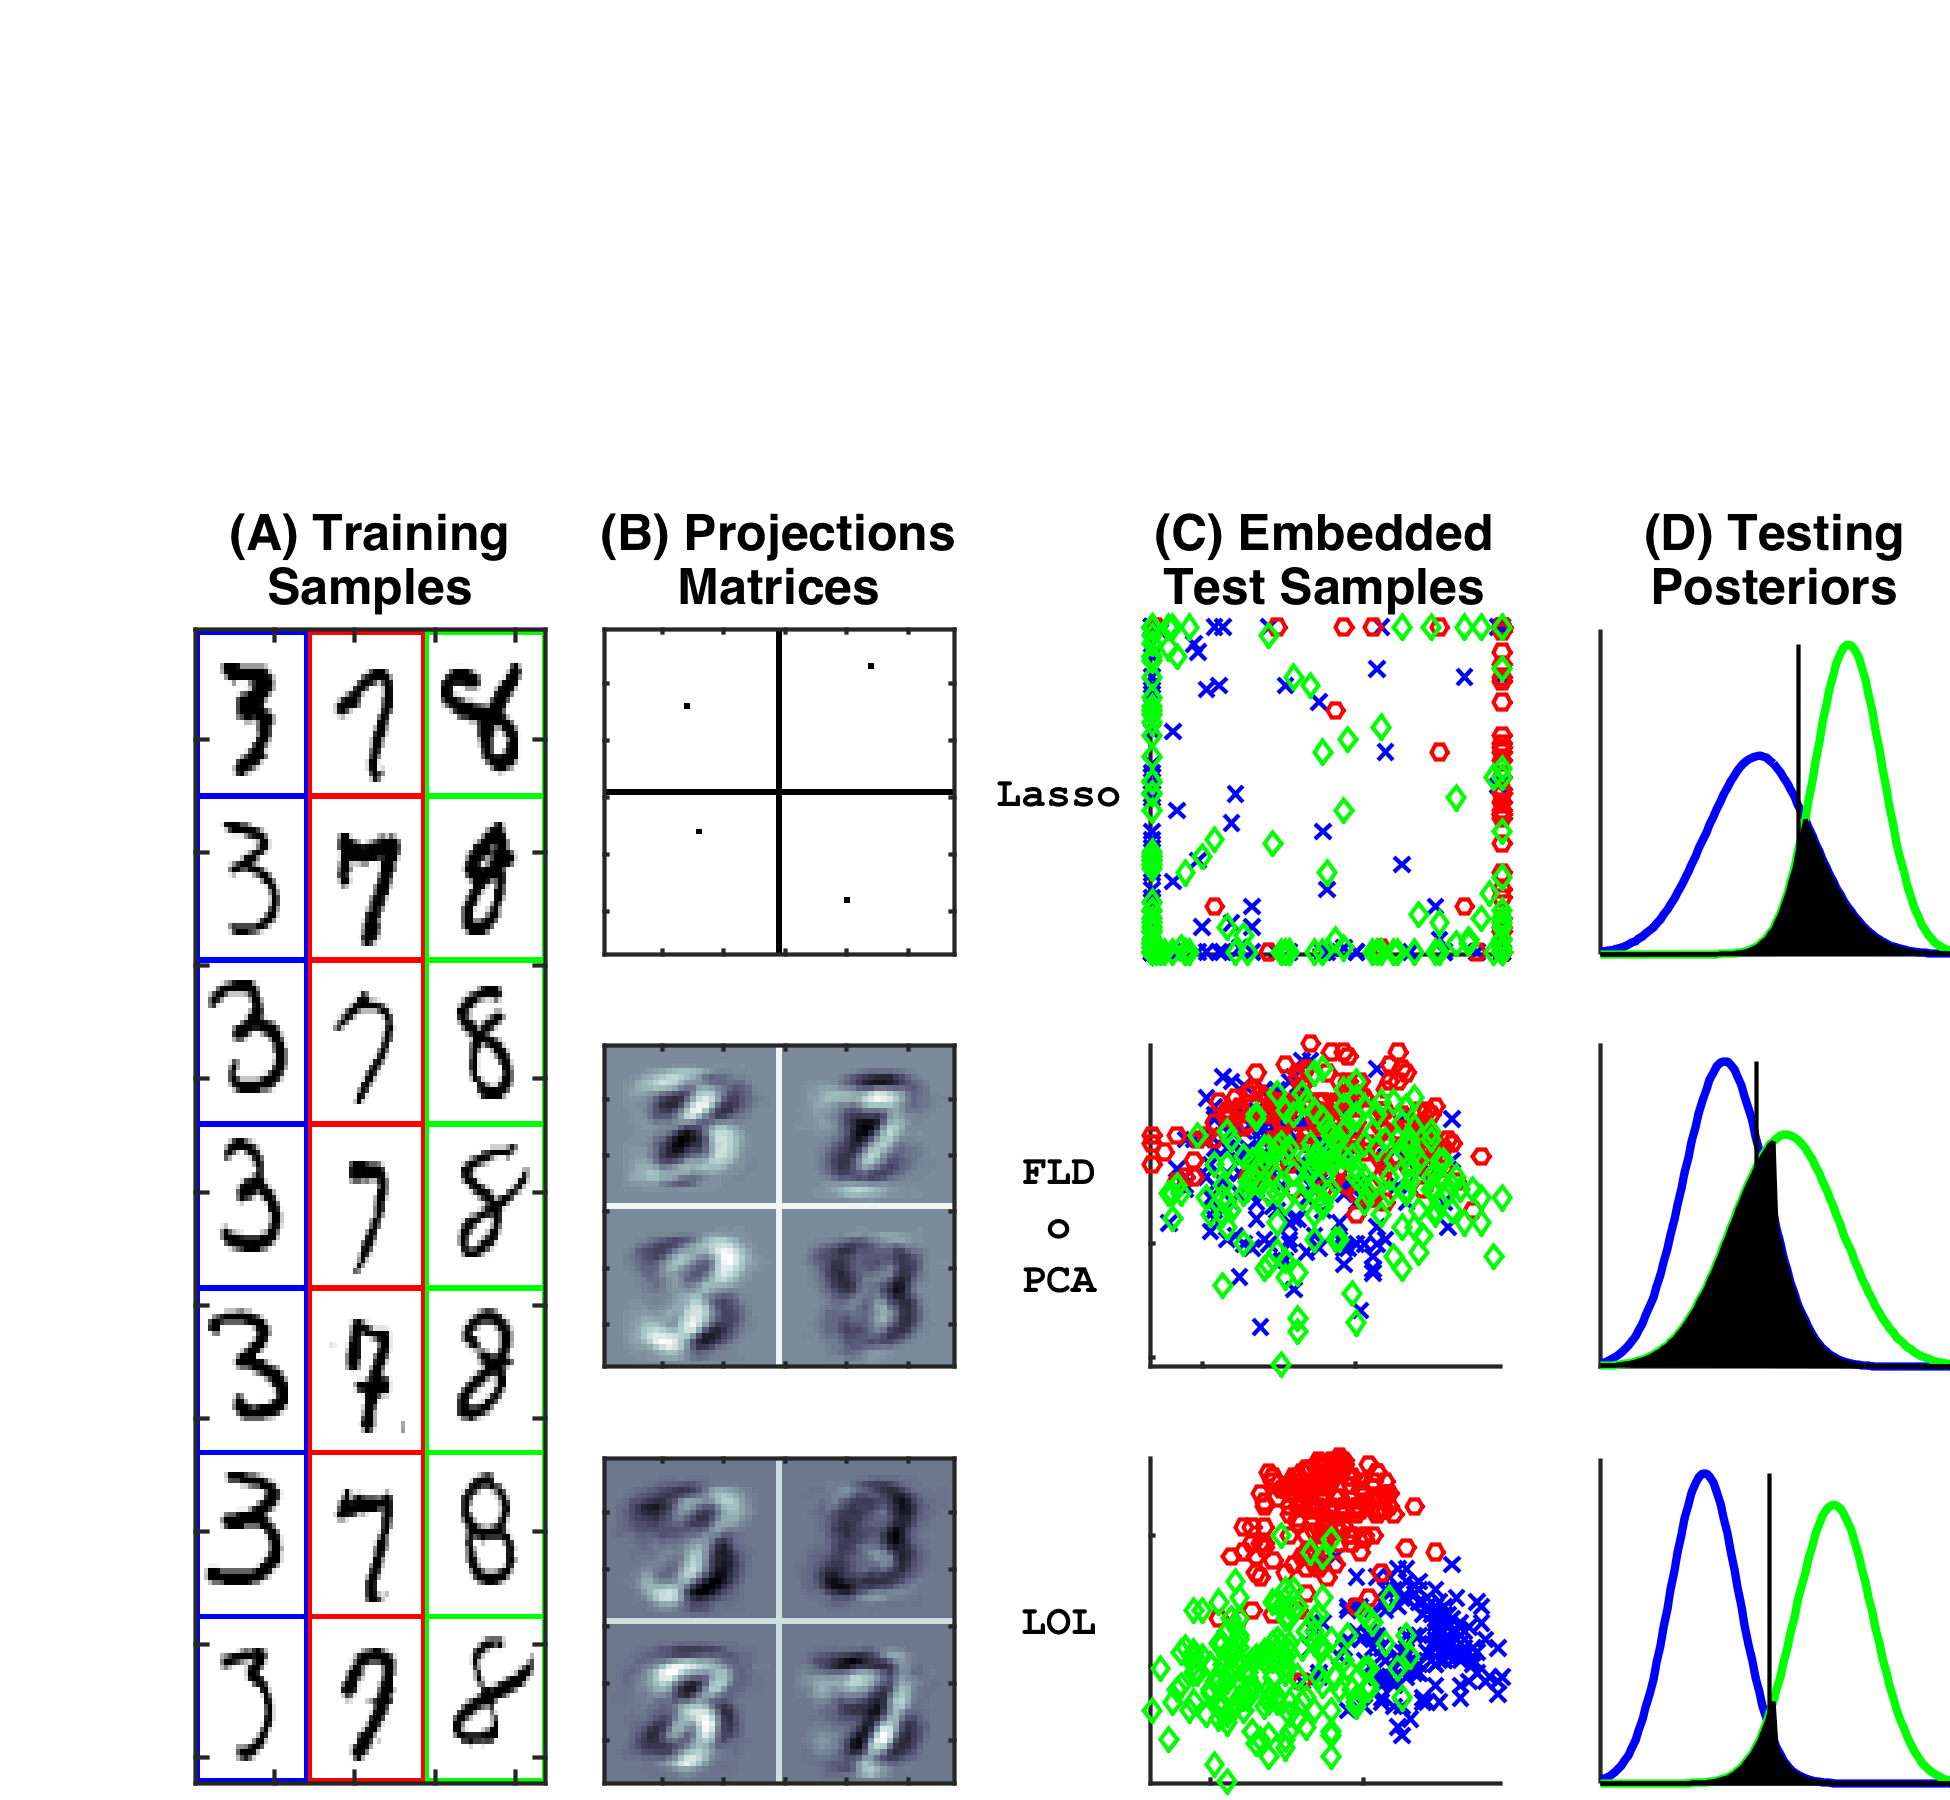
\includegraphics[width=0.7\linewidth,trim=1cm 0cm 0cm 4.0cm,clip=true]{../Figs/mnist}
\caption{
Illustrating three different classifiers---\sct{Lasso}~(top), \sct{Fld$\circ$Pca}~(middle), and \Lol~(bottom)---for embedding images of the digits 3, 7, and 8 (from MNIST), each of which is 28 $\times$ 28 = 784 dimensional.
\textbf{(A)} Exemplars, boundary colors are only for visualization purposes.
\textbf{(B)} The first four projection matrices learned by the three different approaches on 300 training samples. Note that \sct{Lasso}~is sparse and supervised, \Pca~is dense and unsupervised, and \Lol~is dense and supervised.
\textbf{(C)} Embedding 500 test samples into the top 2 dimensions using each approach.  Digits color coded as in (A).
\textbf{(D)}  The estimated posterior distribution of test samples after
5-dimensional projection learned via each method.
We show only 3 vs.~8 for simplicity.
The vertical line shows the classification threshold.
The filled area is the estimated error rate: the goal of any classification algorithm is to minimize that area.
Clearly, \Lol~exhibits the best separation after embedding, which results in the best classification performance.
}
\label{f:mnist}
% \end{wrapfigure}
\end{figure}

Pseudocode of any method that embeds wide data as part of classification proceeds as schematized in Figure \ref{f:mnist}:
(A) obtain/select $n$ training samples of the data,
(B) learn a low dimensional projection,
(C) project $m$ testing samples onto the lower dimensional space,
(D) classify the embedded testing samples using some classifier.
We consider  three different linear dimensionality reduction methods---\sct{Lasso}, \Pca, and \Lol---each of which we compose with a classifier to form high-dimensional classifiers.\footnote{Although \sct{Lasso}~is not a 2-step method (where embedding is learned first, and then a classifier is applied), adaptive lasso \cite{Zou2006a} and its variants improve on lasso's theoretical and empirical properties, so we consider such an approach here.}

To demonstrate the utility of \Lol, we  first consider one of the most popular benchmark datasets ever, the MNIST dataset \cite{mnist}.  This dataset consists of many thousands of examples of images of the digits 0 through 9.  Each such image is represented by a 28$\times$28 matrix, which means that the observed (or ambient) dimensionality of the data is $p=784$.  Because we are motivated by the $n \ll p$ scenario, we subsample the data to select $n=300$ examples of the numbers $3$, $7$, and $8$. We then apply all three approaches to this subsample of the MNIST dataset, learning a projection, and embedding $m=500$ testing samples, and classifying the resulting embedded data.

% Figure \ref{f:mnist}(A) shows several examples of digit, the border of each digit is colored for visualization purposes only.
% Figure \ref{f:mnist}(B) shows the estimated projection matrices for each approach (see Methods for details).
% These are the matrices that transform the data into a low-dimensional representation.



% Figure \ref{f:mnist}(C) shows n'=500 randomly selected training samples from the digits 3, 7, and 8, embedded into the first two dimensions using each of the three approaches. The colors of the embedded points correspond to those in the leftcolumn, that is, 3 is blue, 7 is red, and 8 is green.
% FIgure \ref{f:mnist}(D) shows a smoothed histogram of the posterior probabilities of each test samples after classifying.
\sct{Lasso}, by virtue of being a sparse method, finds the pixels that most discriminate the 3 classes.  The resulting embeddings mostly live along the boundaries, because these images are close to binary, and therefore, images either have or do not have a particular pixel. Indeed, although the images themselves are nearly sparse (over 80\% of the pixels in the dataset have intensity $\leq 0.05$),  a low-dimensional discriminant boundary does not seem to be sparse.  \Pca, on the other hand, finds the linear combinations of training samples that maximize the variance.  This unsupervised linear manifold learning method results in projection matrices that indeed look like linear combinations of the three different digits.  The goal here, however, is separating classes, not maximizing variability.  The resulting embeddings are not particularly well separated, suggesting the the directions of discriminability are not the same as the directions of maximum variance.  \Lol~is our newly proposed supervised linear manifold learning method (see below for details).  The projection matrices it learns look qualitatively much like those of \Pca. This is not surprising, as both are linear combinations of the training examples.  The resulting embeddings however, look quite different.  The three different classes are very clearly separated by even the first two dimensions.  The result of these embeddings yields classifiers whose performance is obvious from looking at the embeddings: \Lol~achieves significantly smaller error than the other two approaches.
This numerical experiment justifies the use of supervised linear manifold learning, we next investigate the performance of these methods in simpler simulated examples, to better illustrate when we can expect \Lol~to outperform other methods, and perhaps more importantly, when we expect this ``vanilla'' variant of \Lol~to fail.

% \clearpage
\subsection*{Linear Gaussian Intuition}

The above real data example suggests the geometric intuition for when \Lol~outperforms its sparse and unsupervised counterparts.  To further investigate, both theoretically and numerically, we consider the simplest setting that illustrates the relevant geometry.  In particular, we consider a two-class classification problem, where both classes are distributed according to a multivariate normal distribution, the class priors are equal, and the joint distribution is centered, so that the only difference between the classes is their means (we call this the Linear Discriminant Analysis (\Lda) model; see Methods for details).




To motivate \Lol, and the following simulations, lets consider what the optimal projection would be in this scenario. The optimal low-dimensional projection is analytically available as the dot product of the difference of means and the inverse covariance matrix, $\mb{A}_*=\mb{\delta}\T \bSig^{-1}$ \cite{Bickel2004a} (see Methods for details).
\Pca, the dominant unsupervised manifold learning method, utilizes only the covariance structure of the data, and ignores the difference between the means.
In particular, \Pca~would project the data on the top d eigenvectors of the  covariance matrix.
\textbf{The key insight of our work is the following: we can combine the difference of the means and the covariance matrix in a simple fashion, rather than just the covariance matrix, to find a low dimensional projection.}
Nai\"vely, this should typically improve performance, because in this stylized scenario, both are important. The \sct{F2M} literature has a similar insight, but a different construction that requires the dimensionality to be smaller than the sample size.  Formally, we implement our idea by simply concatenating the difference of the means with the top d eigenvectors of the  covariance.
This is equivalent to first projecting onto the difference of the means vector, and then projecting the residuals onto the first d principle components.
Thus, it requires almost no additional computational time or complexity over that of \Pca, rather, merely estimates the difference of the means.
In this sense, \Lol~can be thought of as a very simple  ``supervised \Pca''.



\begin{figure}%{R}{0.7\textwidth}%[h!]
% \begin{SCfigure}
\centering
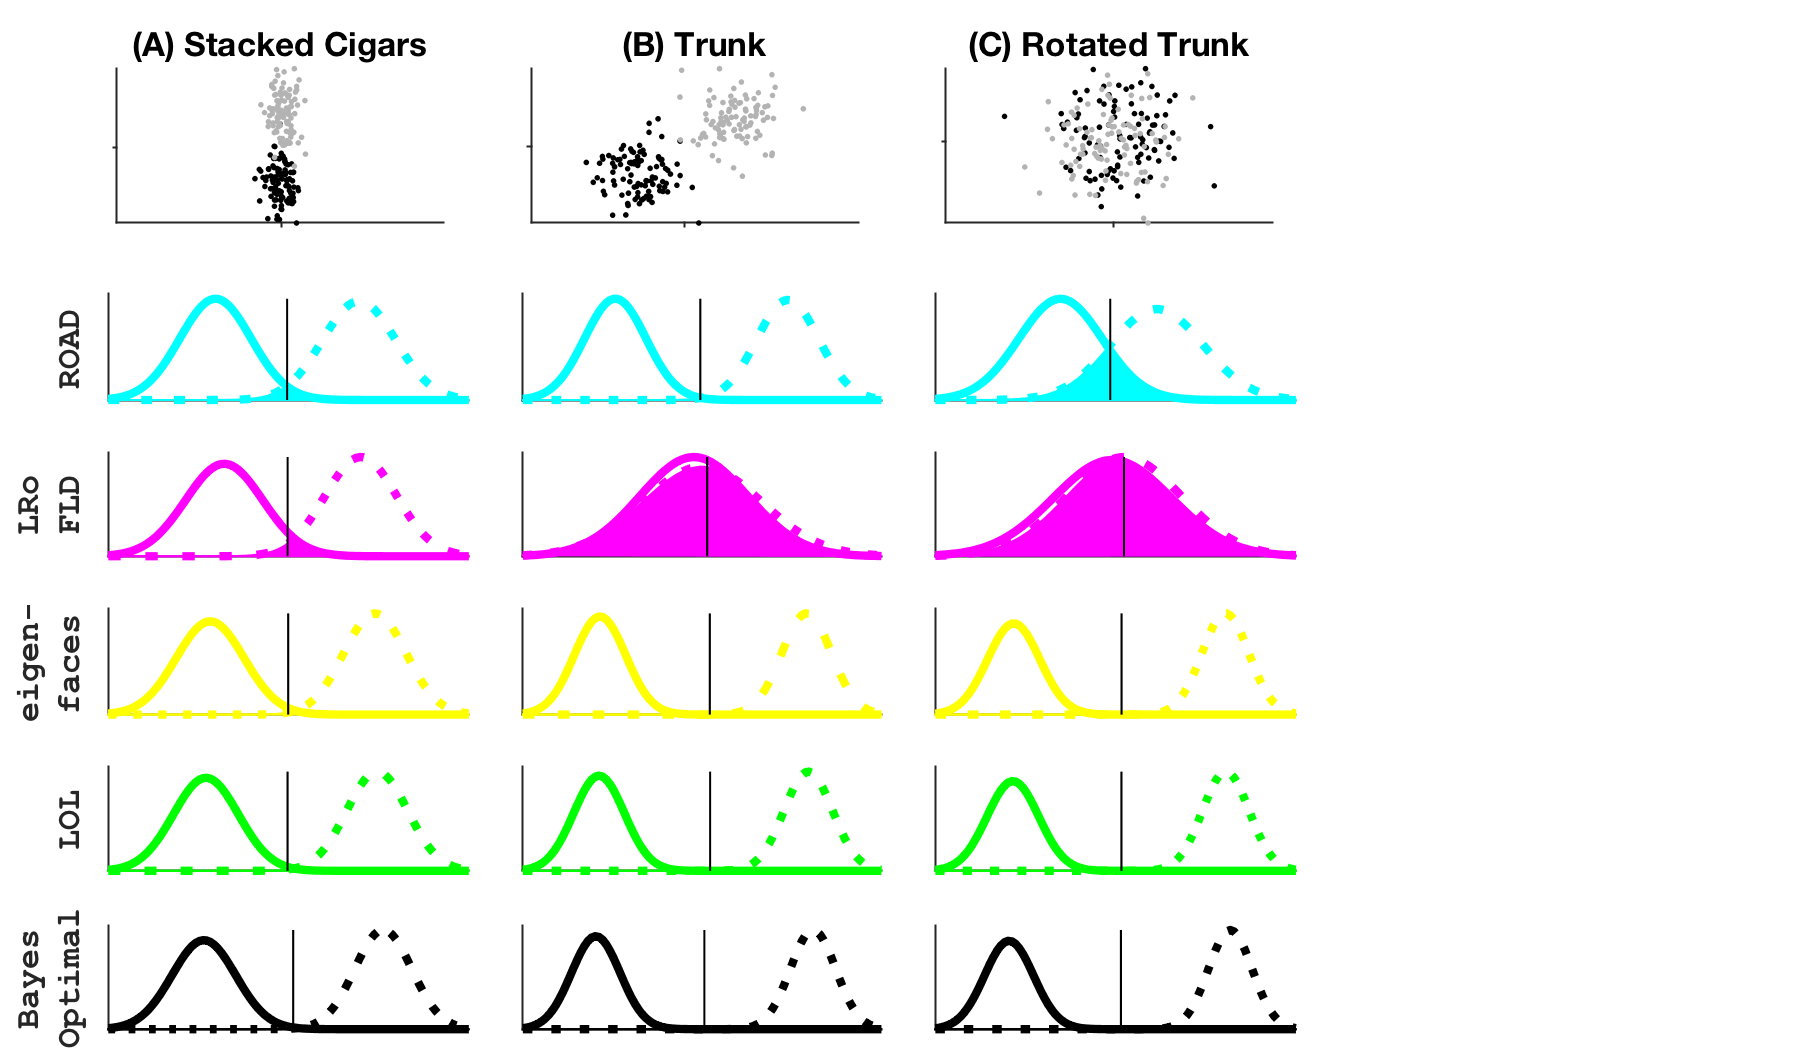
\includegraphics[width=0.8\linewidth,trim=0in 0in 1.5in 0in,clip=true]{../Figs/cigars_est}%l b r t
\caption{
\Lol~achieves near optimal performance for a wide variety of distributions.
Each point is sampled from a multivariate Gaussian;
the three columns correspond to different simulation parameters (see Methods for details).
In each of 3 simulations, we sample $n=100$ points in $p=1000$ dimensions.  And for each approach, we embed into the top 20 dimensions. Note that we use the sample estimates, rather than the true population values of the parameters.  In this setting, the results are  similar.
\textbf{(A)} The mean difference vector is aligned with the direction of maximal variance, maxing it ideal for both \Pca~to discover the discriminant direction and a sparse solution.
\textbf{(B)} The mean difference vector is orthogonal to the direction of maximal variance, making \Pca~fail, but sparse methods can still recover the correct dimensions.
\textbf{(C)} Same as (B), but the data are rotated.
\textbf{Row 1}: A scatter plot of the first two dimensions of the sampled points, with class 0 and 1 as black and gray dots, respectively.
\textbf{Row 2} \sct{Fld $\circ$ Pca}.
\textbf{Row 3} \sct{Road}, a sparse method designed specifically for this model \cite{Fan2012a}.
\textbf{Row 4} \Lol, our newly proposed method.
\textbf{Row 5} the Bayes optimal classifier, which is what all classifiers strive to achieve.
Note that \Lol~is closest to Bayes optimal in all three settings.
}
\label{f:cigars}
\end{figure}
% \vspace{-30pt}


Figure \ref{f:cigars} shows three different examples of data sampled from the \Lda~model to geometrically illustration this intuition.
In each, we sample $n=100$ training samples in $p=1000$ dimensional space, so $n \ll p$.
Figure \ref{f:cigars}(A) shows an example we call  ``stacked cigars''.
In this example and the next, the covariance matrix is diagonal, so all ambient dimensions are independent of one another.
Moreover,  the difference between the means and direction of maximum variance are both large along the same dimensions (they are highly correlated with one another).
This is an idealized setting for \Pca, because \Pca~finds the direction of maximal variance, which happens to correspond to the direction of maximal separation.
However, in the face of high-dimensional data, \Pca~does not weight the discriminant directions sufficiently, and therefore performs only moderately well.\footnote{When having to estimate the eigenvector from the data, \Pca~performs even worse.  This is because when $n \ll p$, \Pca~is an inconsistent estimator with large variance \cite{Baik2006a,Paul2007a}}
Because all dimensions are independent, this is a good scenario for sparse methods.
Indeed,  \sct{Road}, a sparse classifier designed for precisely this scenario,  does an excellent job finding the most useful ambient dimensions.
\Lol~does the best of all three approaches, by using both the difference of the means and the covariance.


Figure \ref{f:cigars}(B) shows an example which is a worst case scenario for using \Pca~to find the optimal projection for classification.
In particular, the variance is getting larger for subsequent dimensions, $\sigma_1 < \sigma_2 < \cdots < \sigma_p$, while the magnitudes of the difference between the means are decreasing with dimension, $\delta_1 > \delta_2 < \cdots > \delta_p$.
Thus, for any truncation level,  \Pca~finds exactly the \emph{wrong} directions.
\sct{Road} is not hampered by this problem, it is also able to find the directions of maximal discrimination, rather than those of maximal variance.
Again, \Lol, by using both parameters, does extremely well.


Figure \ref{f:cigars}(C) is exactly the same as (B), except the data have been randomly rotated in all 1000 dimensions.  This means that none of the original coordinates have much information, rather, linear combinations of them do.
This is evidenced by observing the scatter plot, which shows that two dimensions clearly fail to disambiguate the two classes.
\Pca, being rotationally invariant, fails in this scenario as it did in (B).
Now, there is no small number of ambient dimensions that separate the data well, so \sct{Road} also fails.
 \Lol is unperturbed by this rotation; in particular, it is able to ``unrotate'' the data, to find dimensions that optimally separate the two classes.


\subsection*{Theoretical Confirmation}

The above numerical experiments provide the intuition to guide our theoretical developments.
\begin{thm} \label{t:LDA}
Under the \Lda~model, \Lol~is better than \Pca.
\end{thm}
In words, it is better to incorporate the mean difference vector into the projection matrix.  The degree of improvement is a function of the embedding dimension d, the ambient dimensionality p, and the parameters (see Methods for details and proof).



\subsection*{How many dimensions to keep?}

In the above numerical and theoretical investigations, we fixed $d$, the number of dimensions to embed into.  Much unsupervised manifold learning theory typically focuses on finding the ``true'' intrinsic dimensionality of the data.   The analogous question for supervised manifold learning would be to find the true intrinsic dimensionality of the discriminant boundary.  However, in real data problems, typically, their is no perfect low dimensional representation because of noise.
% , rather, the more data we obtain, the higher-dimensional discriminant boundary we can estimate, and the close to Bayes optimal we can perform.

Thus, in all the following simulations, the true ambient dimensionality of the data is equal to the dimensionality of the optimal discriminant boundary (given infinite data).  In other words, there does not exist a discriminant space that is lower dimensional than the ambient space, so we cannot find the ``intrinsic dimension'' of the data or the discriminant boundary.  Rather, we face a trade-off: keeping more dimensions reduces bias, but increases variance.  The optimal bias/variance trade-off depends on the distribution of the data, as well as the sample size \cite{Trunk1979a}.

% We formalize this notion for the \Lda model and proof the following:
% \begin{thm} \label{t:n}
% Under the \Lda~ model, estimated \Lol~is better than \Pca.
% \end{thm}
% Note that the degree of improvement is a function of the number of samples $n$, in addition to the embedding dimension $d$, the ambient dimensionality $p$, and the parameters (see Methods for details and proof).


Consider again the rotated trunk example as well as a ``Toeplitz'' example, as depicted in Figures \ref{f:properties}(A) and (B), respectively.  In both cases, the data are sampled from the \Lda~ model, and in both cases, the optimal dimensionality under finite samples depends on the particular approach, but is never the true dimensionality.  Moreover, \Lol~dominates the other approaches, regardless of the number of dimensions used.
%
Figure \ref{f:properties}(C) shows a sparse example with ``fat tails'' to mirror real data settings better.  The qualitative results are consistent with those of (A) and (B), even though the setting is no longer exactly the setting under which we have theoretical confirmation.

% Indeed, we can generalize Theorem \ref{t:n} to include ``sub-Gaussian'' data, rather than just Gaussian:
% \begin{thm} \label{t:FAT}
% Under a sub-Gaussian generalization of the \Lda~ model, \Lol~is still better than \Pca.
% \end{thm}

\subsection*{Multiple Classes}

\Lol~can trivially be extended to $>2$ class situations.  Nai\"vely it may seem like we would need to keep all pairwise differences between means.  However, given $k$ classes, the set of all $k^2$ differences is only rank $k-1$.  In other words, we can equivalently find the class which has the maximum number of samples (breaking ties randomly), and subtract its mean from all other class means.  Figure \ref{f:properties}(D) shows a 3-class generalization of (A).  While \Lol~uses the additional class naturally,  many previously proposed high-dimensional \Fld~variants, such as \sct{Road}, natively only work for 2-classes.


\begin{figure}[h!]
\centering
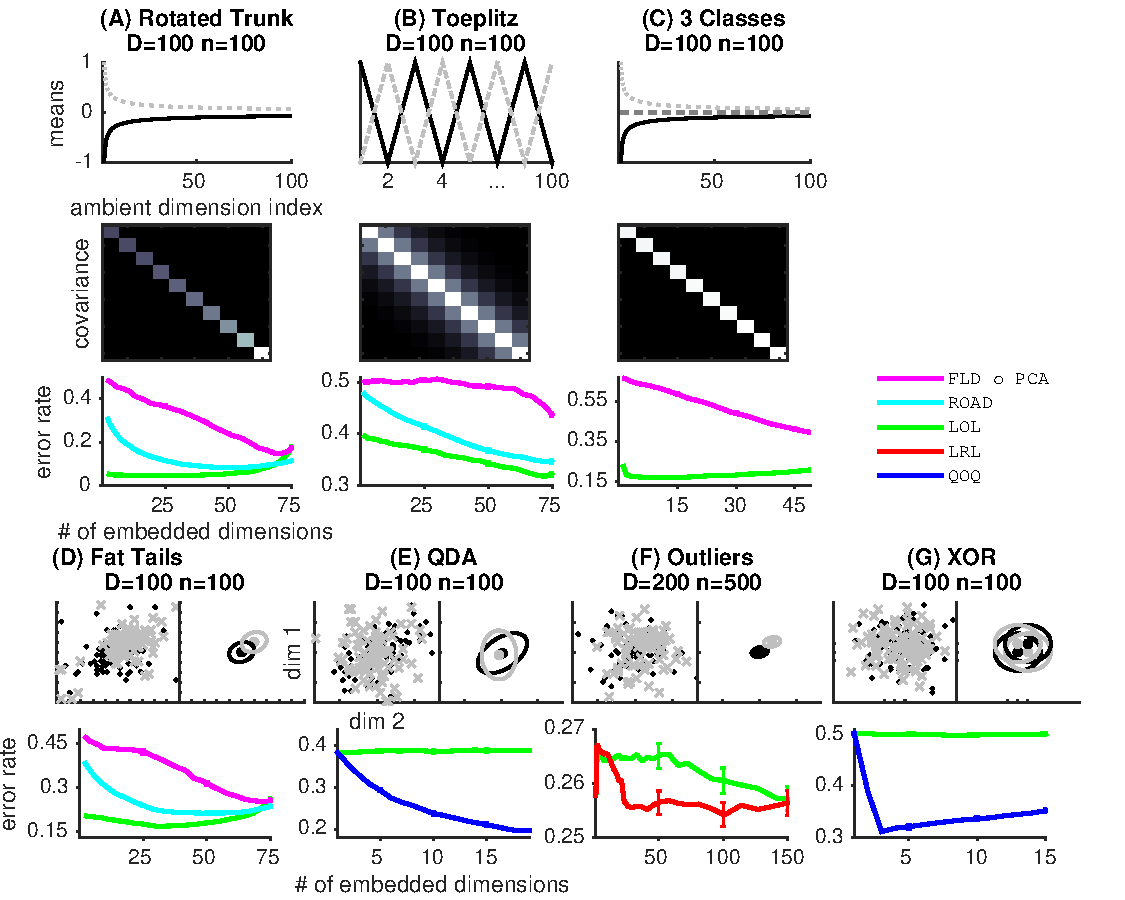
\includegraphics[width=1\linewidth]{../Figs/properties}
\caption{
Seven simulations demonstrating that even when the true discriminant boundary is high-dimensional, \Lol~can find a low-dimensional projection that wins the bias-variance trade-off against competing methods.
For the first four, the top panels depict the means (top), the shared covariance matrix (middle).  For the next three, the top panels depict a 2D scatter plot (left), mean and level set of one standard deviation of covariance matrix (right).  For all seven simulations, the bottom panel shows misclassification rate as a function of the number of embedded dimensions, for several different classifiers.  The simulations settings are as follows:
\textbf{(A)} Rotated Trunk: same as Figure \ref{f:cigars}(C).
\textbf{(B)} Toeplitz: another setting where mean difference is not well correlated with any eigenvector, and no ambient coordinate is particularly useful on its own.
\textbf{(C)} 3 Classes: \Lol~naturally adapts to multiple classes.
\textbf{(D)} Fat Tails: a common phenomenon in real data that is more general than our theory supports.
\textbf{(E)} QDA: QOQ, a variant of \Lol~when each class has a unique covariance, outperforms \Lol, as expected.
\textbf{(F)} Outliers: adding high-dimensional outliers degrades performance of standard eigensolvers, but those can easily be replaced in \Lol~for a robust variants (called \Lrl).
\textbf{(F)} XOR: a high-dimensional stochastic generalization of XOR, demonstrating the \Lol~and QOQ work even in scenarios that are quite distinct from the original motivating problems.
In all 7 cases, \Lol, or the appropriate generalization thereof, outperforms unsupervised, sparse, or other methods.  Moreover, the optimal embedding dimension is never the true discriminant dimension, but rather, a smaller number jointly determined by parameter settings and sample size.
}
\label{f:properties}
\end{figure}



\subsection*{Generalizations of \Lol}

The simple geometric intuition which led to the development of \Lol~suggests that we can easily generalize \Lol~to be more appropriate for more complicated settings. We consider three additional scenarios:

\para{QDA} Sometimes, it makes more sense to model each class as having a unique covariance matrix, rather than a shared covariance matrix.  Assuming everything is Gaussian, the optimal classifier in this scenario is called  Quadratic Discriminant Analysis (QDA) \cite{Hastie2004}.  Intuitively then, we can modify \Lol~to compute the eigenvectors separately for each class, and concatenate them (sorting them according to their singular values).  Moreover, rather than classifying the projected data with \Lda, we can then classify the projected data with QDA.  Indeed, simulating data according to such a model (Figure \ref{f:properties}(E)), \Lol~performs slightly better than chance, regardless of the number of dimensions we use to project, whereas QOQ (which denotes we estimate eigenvectors separately and then use QDA on the projected data) performs significantly better regardless of how many dimensions it keeps.

\para{Outliers}  Outliers persist in many real data sets.  Finding outliers, especially in high-dimensional data, is both tedious and difficult.  Therefore, it is often advantageous to have estimators that are robust to certain kinds of outliers \cite{Huber1981a,Rousseeuw1999a,Ferrari2010a}.  \Pca~and eigenvector computation are particularly sensitive to outliers \cite{Candes2009b}.  Because \Lol~is so simple and modular, we can replace typical eigenvector computation with a robust variant thereof, such as the geometric median subspace embedding \cite{Zhang2014a}.  Figure \ref{f:properties}(F) shows an example where we generated  $n/2$ training samples according to the simple \Lda~ model, but then added another $n/2$ training samples from a noise model.  \Lrl~(our robust variant of \Lol~that simply replaces the fragile eigenvector computation with a robust version), performs better than \Lol~regardless of the number of dimensions we keep.

\para{XOR}  XOR is perhaps the simplest nonlinear problem, the problem that led to the demise of the perceptron, prior to its resurgence after the development of multi-layer perceptrons \cite{Bishop2006a}.  Thus, in our opinion, it is warranted to check whether any new classification method can perform well in this scenario.  The classical (two-dimensional) XOR problem is quite simple: the output of a classifier is zero if both inputs are the same (00 or 11), and the output is one if the inputs differ (01 or 10).  Figure \ref{f:properties}(G) shows a high dimensional and stochastic variant of XOR.  This simulation was designed such that standard classifiers, such as support vector machines and random forests, achieve chance levels (not shown).  \Lol, performs moderately better than chance, and QOQ performs significantly better than chance, regardless of the chosen dimensionality.  This demonstrates that our classifiers developed herein, though quite simple and intuition, can perform well even in settings where the data are badly modeled by our underlying assumptions.  This mirrors previous findings where the so-called ``idiots's Bayes'' classifier outperforms more sophisticated classifiers \cite{Bickel2004a}.  In fact, we think of our work as finding intermediate points between idiot's Bayes (or nai\"ve Bayes) and \Fld, by enabling degrees of regularization by changing the dimensionality used.


\subsection*{Computational Efficiency}

In many applications, the main quantifiable consideration in whether to use a particular method, other than accuracy, is computational efficiency.  Because implementing \Lol~requires only highly optimized linear algebraic routines---including computing moments and singular value decomposition---rather than the costly iterative programming techniques currently required for sparse or dictionary learning type problems.  To quantify the computational efficiency of \Lol~and its variants, Figure \ref{f:speed} shows the wall time it takes to run each method on the stacked cigars problem, varying the ambient dimensionality, embedded dimensionality, and sample size.  Note that for completeness, we include two additional variants of \Lol: \Lal~and \Lfl.  \Lfl~(short for Linear Fast Low-rank) replaces the standard \Svd~algorithm with a randomized variant, which can be much faster in certain situations \cite{Halko2011a}.  \Lal~(short for Linear Approximate Low-rank) goes even one step further, replacing \Svd~with random projections \cite{Candes2006a}.  This variant of \Lol~is the fastest, its runtime is  least sensitive to $(p,d,n)$, and its accuracy is often commensurate (or better) than other variants of \Lol.  The runtime of all the variants of \Lol~are quite similar to \sct{Fld $\circ$ Pca}.  Given, given \Lol's improved accuracy, and nearly identical simplicity, it seems there is very little reason to not use \Lol~instead of \sct{Fld $\circ$ Pca}.

\begin{figure}[h!]
\centering
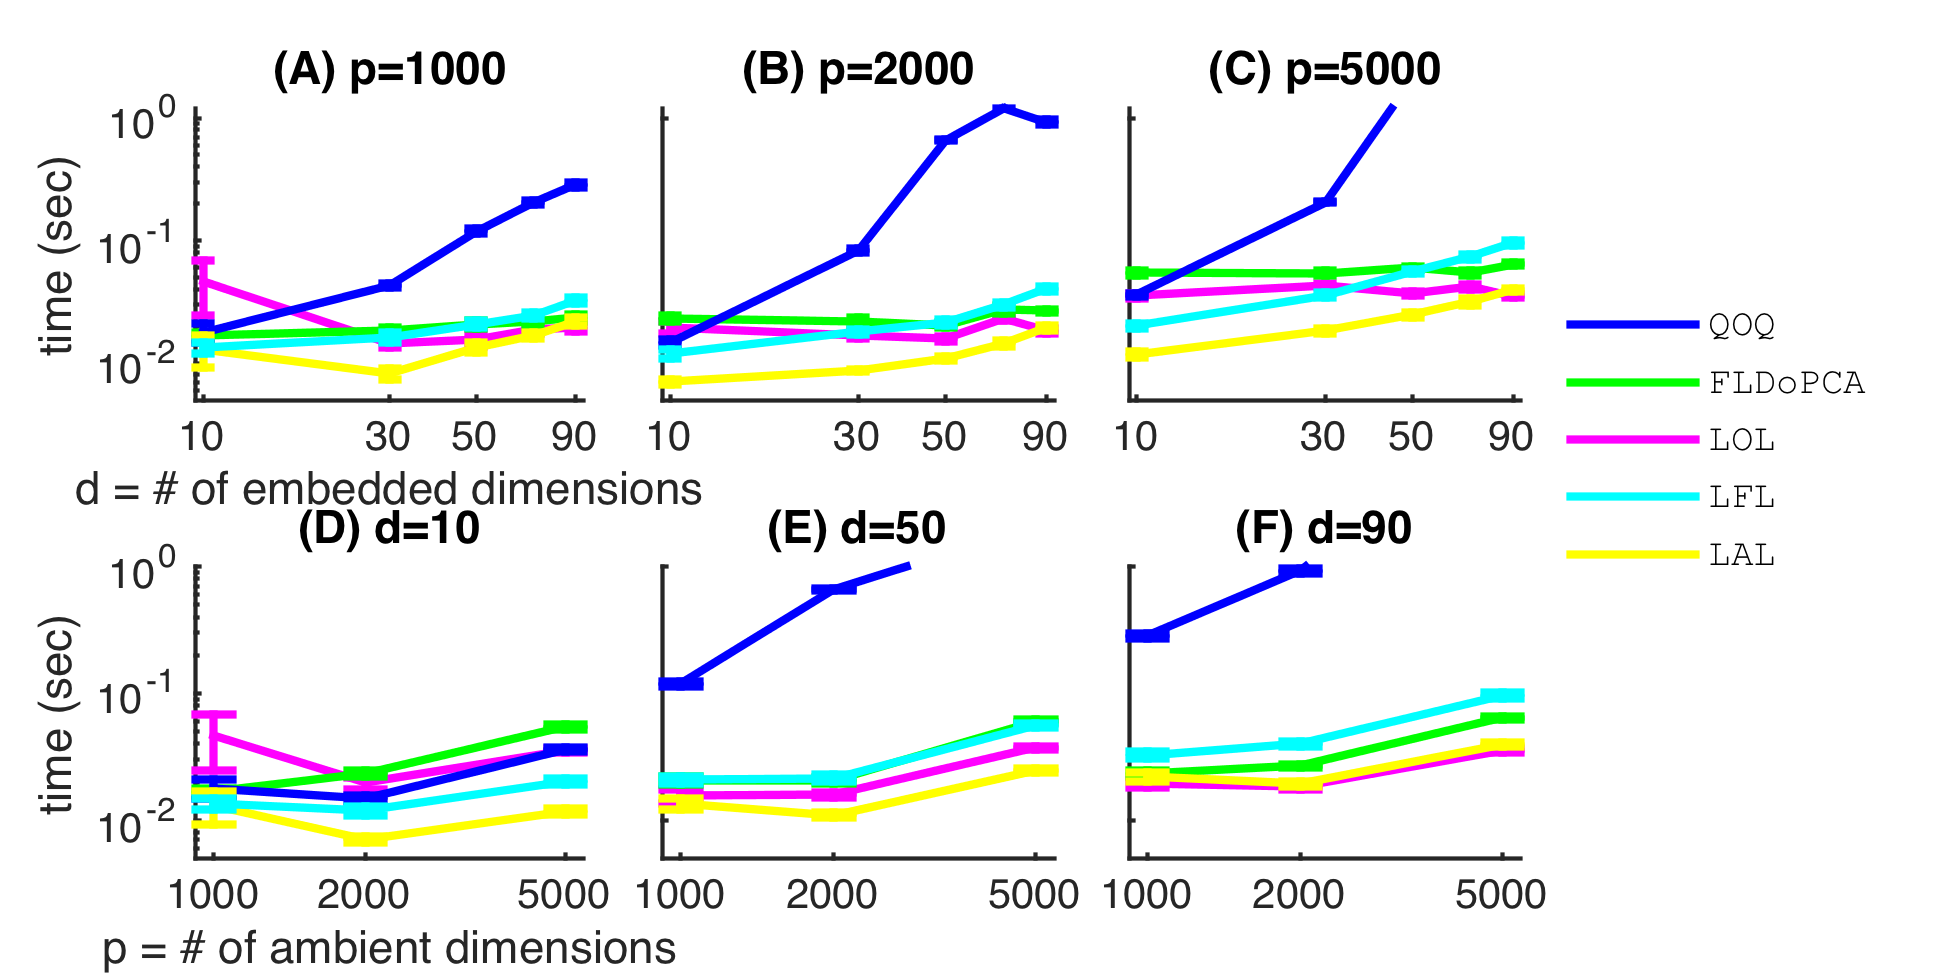
\includegraphics[width=1\linewidth]{../Figs/speed_test}
\caption{
Computational efficiency of various low-dimensional projection methods. In all cases, $n=100$, and we used the ``stacked cigars'' simulation parameters.   We compare \Pca~with the projection steps from \Lol, \Qoq, \Lrl, \Lfl, and \Lal, for different values of $(p,d)$.  The addition of the mean difference vector is essentially negligible.  Moreover, for small $d$, the \Lfl~is advantageous.  \Lal~is always fastest, and its performance is often comparable to other methods (not shown).
}
\label{f:speed}
\end{figure}




\subsection*{Benchmark Real Data Applications}


To more comprehensively understand the relative advantages and disadvantages of \Lol~with respect to other high-dimensional classification approaches, in addition to evaluating its performance in theory, and in a variety of numerical simulations,
 it is important to evaluate it also on benchmark datasets.  For these purposes, we have selected four commonly used high-dimensional datasets (see Methods for details).  For each, we compare \Lol~to (i) support vector machines (SVM), (ii) \sct{Road}, (iii) lasso, (iv) and random forest (RF).  Because in practice all these approaches have ``hyperparameters'' to tune, we consider several possible values for  SVM, lasso, and \Lol~(but not RF, as its runtime was too high).  Figure \ref{f:realdata} shows the results for all four datasets.



\begin{figure}
\centering
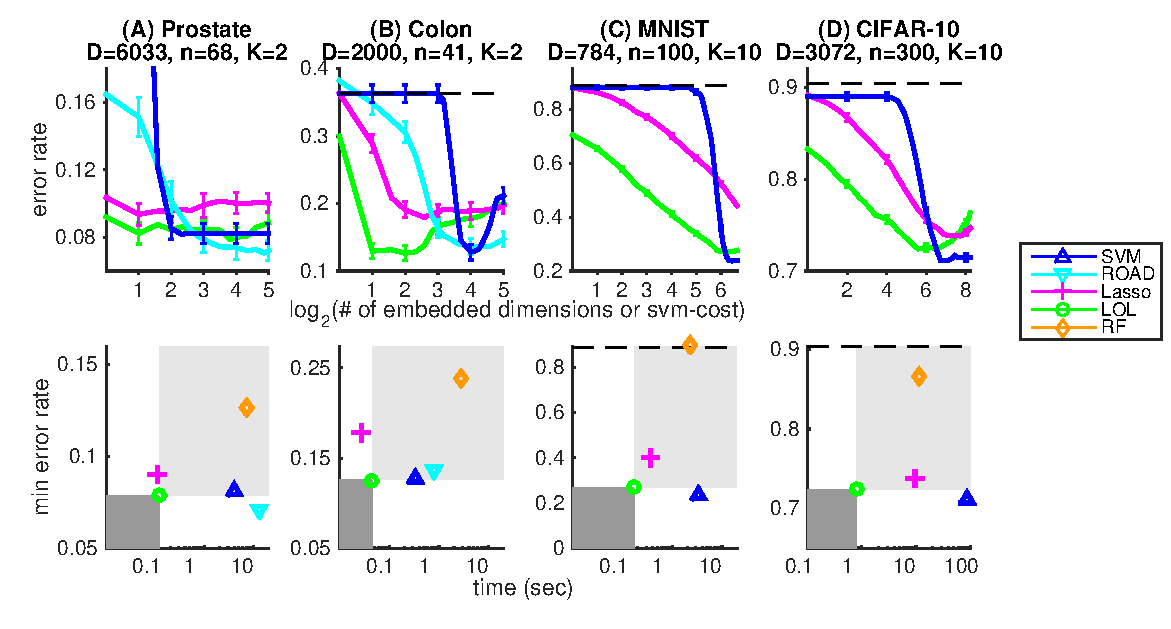
\includegraphics[width=1\linewidth]{../Figs/realdata}
\caption{
For four standard datasets, we benchmark \Lol~(green circles) versus standard classification methods, including support vector machines (blue up triangles), \sct{Road} (cyan down triangles), \sct{Lasso}~(magenta pluses), and random forest (orange diamonds).
Top panels show error rate as a function of log$_2$ number of embedded dimensions (for \Lol, \sct{Road}, and \sct{Lasso}) or cost (for SVM).
% \Lol~consistently achieves lower error for fewer dimensions.
Bottom panels show the minimum error rate achieved by each of the five algorithms versus time.
The lower left dark gray (upper right light gray) rectangle is the area in which any algorithm is \emph{better}  (worse) than \Lol~in terms of both accuracy and efficiency.
\textbf{(A)} Prostate: a standard sparse dataset.  1-dimensional \Lol~does very well, although keeping $2^5$ ambient coordinates slightly improves performance, at a significant cost of compute time (two orders of magnitude), with minimal additional interpretability.
\textbf{(B)} Colon: another standard sparse dataset.  Here, 2-4 dimensions of \Lol~outperforms all other approaches considered.
\textbf{(C)} MNIST: 10 image categories here, so \sct{Road} is not possible.  \Lol~does very well regardless of the number of dimensions kept.  SVN marginally improves on \Lol~accuracy, at a significant cost in computation (two orders of magnitude).
\textbf{(D)} CIFAR-10: a higher dimensional and newer 10 category image classification problem.  Results are qualitatively similar to (C).
%
Note that, for none of the problems is there an algorithm ever performing better and faster than \Lol; rather, most algorithms typically perform worse and slower (though some are more accurate and much more computationally expensive.
This suggests that regardless of how one subjectively weights computational efficiency versus accuracy, \Lol~is the best default algorithm in a variety of real data settings.
}
\label{f:realdata}
\end{figure}



Qualitatively, the results are similar across datasets: \Lol~achieves high accuracy and computational efficiency as compared to the other methodologies.  Considering Figure \ref{f:realdata}(A) and (B), two popular sparse settings, we find that \Lol~can find very low dimensional projections with very good accuracy. For the prostate data, with a sufficiently non-sparse solution for \sct{Road}, it slightly outperforms \Lol, but at substantial computational cost, in particular, \sct{Road} takes about 100 times longer to run on this dataset.   Figure \ref{f:realdata}(C) and (D) are 10-class problems, so \sct{Road} is no longer possible.  Here, SVM can again slightly outperform \Lol, but again, requiring 100 fold additional computational time.  In all cases, the beloved random forest classifier performs subpar.


\subsection*{Extensions to Other Supervised Learning Problems}

The utility of incorporating the mean difference vector into supervised machine learning for wide data extends beyond merely classification.  In particular, hypothesis testing can be considered as a special case of classification, with a particular loss function.  Therefore we apply the same idea to a hypothesis testing scenario.  The multivariate generalization of the t-test, called Hotelling's Test, suffers from the same problem as does the classification problem; namely, it requires inverting an estimate of the covariance matrix. To mitigate this issue in the hypothesis testing scenario, prior art applied similar tricks as they have done in the classification setting. One particularly nice and related example is that of  Lopes et al. \cite{Lopes2011a}, who addresses this dilemma by using random projections to obtain a low-dimensional representation, following by applying Hotelling's Test in the lower dimensional subspace.  Figure \ref{f:generalizations}(A) and (B) shows the power of their test alongside the power of the same approach, but using the \Lol~projection rather than random projections.  The two different simulations include the simulated settings considered in their manuscript (see Methods for details).  The results make it clear that the \Lol~test has higher power for essentially all scenarios.  Moreover, it is not merely the replacing random projections with \Pca (solid magenta line), nor simply incorporating the mean difference vector (dashed green line), but rather, it appears that \Lol~for testing uses both modifications to improve performance.

High-dimensional linear regression is another supervised learning method that can utilize this idea. Linear regression, like classification and Hotelling's Test, requires inverting a singular matrix as well.  By projecting the data only a lower dimensional subspace first, followed by linear regression on the low-dimensional data, we can mitigate the curse of high-dimensions.  To choose the projection matrix, we partition the data into K partitions, based on the percentile of the target variable, we obtain a K class classification problem.  Then, we can apply \Lol~to learn the embedding.  Figure \ref{f:generalizations}(C) shows an example of this approach, contrasted with lasso and partial least squares, in a sparse simulation setting (see Methods for details). \Lol~is able to find a better low-dimensional projection than lasso, and performs significantly better than PLS, for essentially all choices of number of dimensions to embed into.




\begin{figure}
% \begin{wrapfigure}{R}{0.7\textwidth} %[h!]
\centering
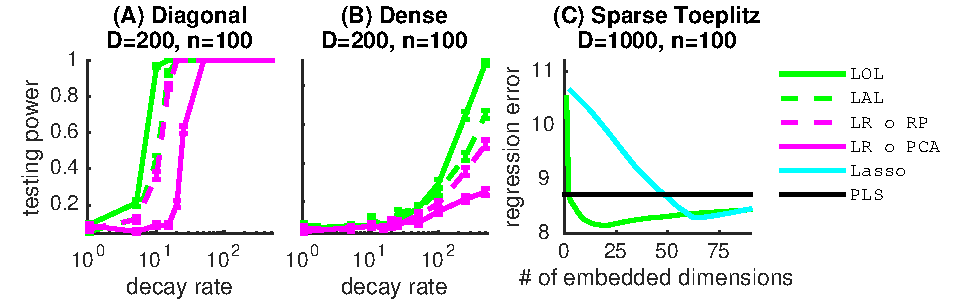
\includegraphics[width=1\linewidth]{../Figs/regression_power}
\caption{
The intuition of including the mean difference vector is equally useful for other supervised manifold learning problems, including testing and regression.
(A) and (B) show two different high-dimensional testing settings, as described in Methods.  Power is plotted against the decay rate of the spectrum, which approximates the effective number of dimensions.  \Lol~composed with Hotelling's test outperforms the random projections variants described in \cite{Lopes2011a}, as well as several other variants.
(C) shows a high-dimensional regression settings, as described in Methods.  Log$_{10}$ mean squared error is plotted against the number of embedded dimensions.
Regression \Lol~composed with linear regression outperforms \sct{Lasso}~(cyan), the classic sparse regression method, as well as partial least squares (PLS; black).
In the legend, 'A' denote either 'linear regression' (in (C)), or 'Hotelling' (in (A) and (B)).
These three simulation settings therefore demonstrate the generality of this technique.
}
\label{f:generalizations}
% \end{wrapfigure}
\end{figure}
% \clearpage


\section*{Discussion}


We have introduced a very simple, yet new, methodology to improve performance on supervised learning problems with wide data.  In particular, we have proposed a supervised manifold learning procedure, the utilizes both the difference of the means, and the covariance matrices.  This is in stark contrast to previous approaches, which only utilize the covariance matrices (or kernel variants thereof), or solve a difficult optimization theoretic problem.  In addition to demonstrating the accuracy and numerical efficiency of \Lol~on simulated and real classification problems, we also demonstrate how the same idea can also be used for other kinds of supervised learning problems, including regression and hypothesis testing. Theoretical guarantees suggest that this line of research is promising and can be extended to other more general settings and tasks.


\subsection*{Qualitative Design Considerations}


Finally, in addition to the above mentioned quantitative criteria, there are also many qualitative criteria that merit consideration at each level of analysis.  For the problem specification level,  the model choices also determine the  \textbf{appropriateness}.  Indeed, real decision criteria are often quite difficult to specify precisely, and so our problem specification is almost always related to but not exactly the problem we hope to achieve.  For example, while we might want to parse a scene, we often tackle a simpler problem of checking whether an object of a particular kind is present because it is easier.  For the algorithm level, the \textbf{interpretability} of the resulting estimator is often an important consideration.  For example, when developing biomarkers, it is important that the doctors and insurance companies can understand the decision making process of the algorithm, otherwise they might not believe the results. For the implementation level,  how \textbf{accessible} is the implementation is crucial.  In particular as more people outside the ivory academic tower---such as citizen scientists and even academics in the developing world---are contributing to data science and scientific discovery in general, access to the implementation is increasingly important.  Finally, at the platform level, the \textbf{ease of use} of the platform is increasingly important.  For example, requiring tedious installations of many different software libraries, or specialized hardware, can make the platform difficult to employ.  

\subsection*{Related Work}

One of the first publications to compose \Fld~with an unsupervised learning method was the celebrated Fisherfaces paper \cite{Belhumeur1997a}.  The authors showed via a sequence of numerical experiments the utility of embedding with \Pca~prior to classifying with \Fld.  We extend this work by adding a supervised component to the initial embedding.  Moreover, we provide the geometric intuition for why and when this is advantageous, as well as show numerous examples demonstrating its superiority.  %Finally, we have matrix concentration inequalities proving the advantages of \Lol~over Fisherfaces.

Such manifold learning methods, while exhibiting both strong theoretical \cite{Eckart1936a,deSilva2003, Allard2012} and empirical performance, are fully unsupervised.  Thus, in classification problems, they discover a low-dimensional representation of the data, ignoring the labels.  This can be highly problematic when the discriminant dimensions and the directions of maximal variance in the learned manifold are not aligned (see Figure \ref{f:mnist} for an example).  Supervised dimensionality reduction techniques, therefore, combine the best of both worlds, explicitly searching for low-dimensional discriminant boundaries.  A set of methods from the statistics community is collectively referred to as   ``sufficient dimensionality reduction'' (SIR) or ``first two moments'' (F2M) methods  \cite{Li1991a, Tishby1999a, Globerson2003a, Cook2005a,Fukumizu2004a}.  These methods are theoretically elegant, but typically require the sample size to be larger than the number of observed dimensions (although see \cite{Cook2013} for some promising work).  Other approaches formulate an optimization problem, such as projection pursuit \cite{Huber1985a}, empirical risk minimization \cite{Belkin2006a}, or supervised dictionary learning \cite{Mairal2009}.  These methods are limited because they are prone to fall into local minima, they require costly iterative algorithms, and lack any theoretical guarantees \cite{Belkin2006a}.   Thus, there remains a gap in the literature: a supervised learning method with theoretical convergence guarantees appropriate when the dimensionality is orders of magnitude larger than the sample size.



\subsection*{Next Steps}

The \Lol~idea, appending the mean difference vector to convert unsupervised manifold learning to supervised manifold learning, has many potential applications.  We have presented the first few.  Incorporating additional nonlinearities via kernel methods \cite{Mika1999a}, ensemble methods such as random forests \cite{Breiman2001a}, multiscale methods \cite{Allard2012},  and more scalable implementations \cite{Chang2011a}, are all of immediate interest.


\clearpage

\begin{figure}
\centering
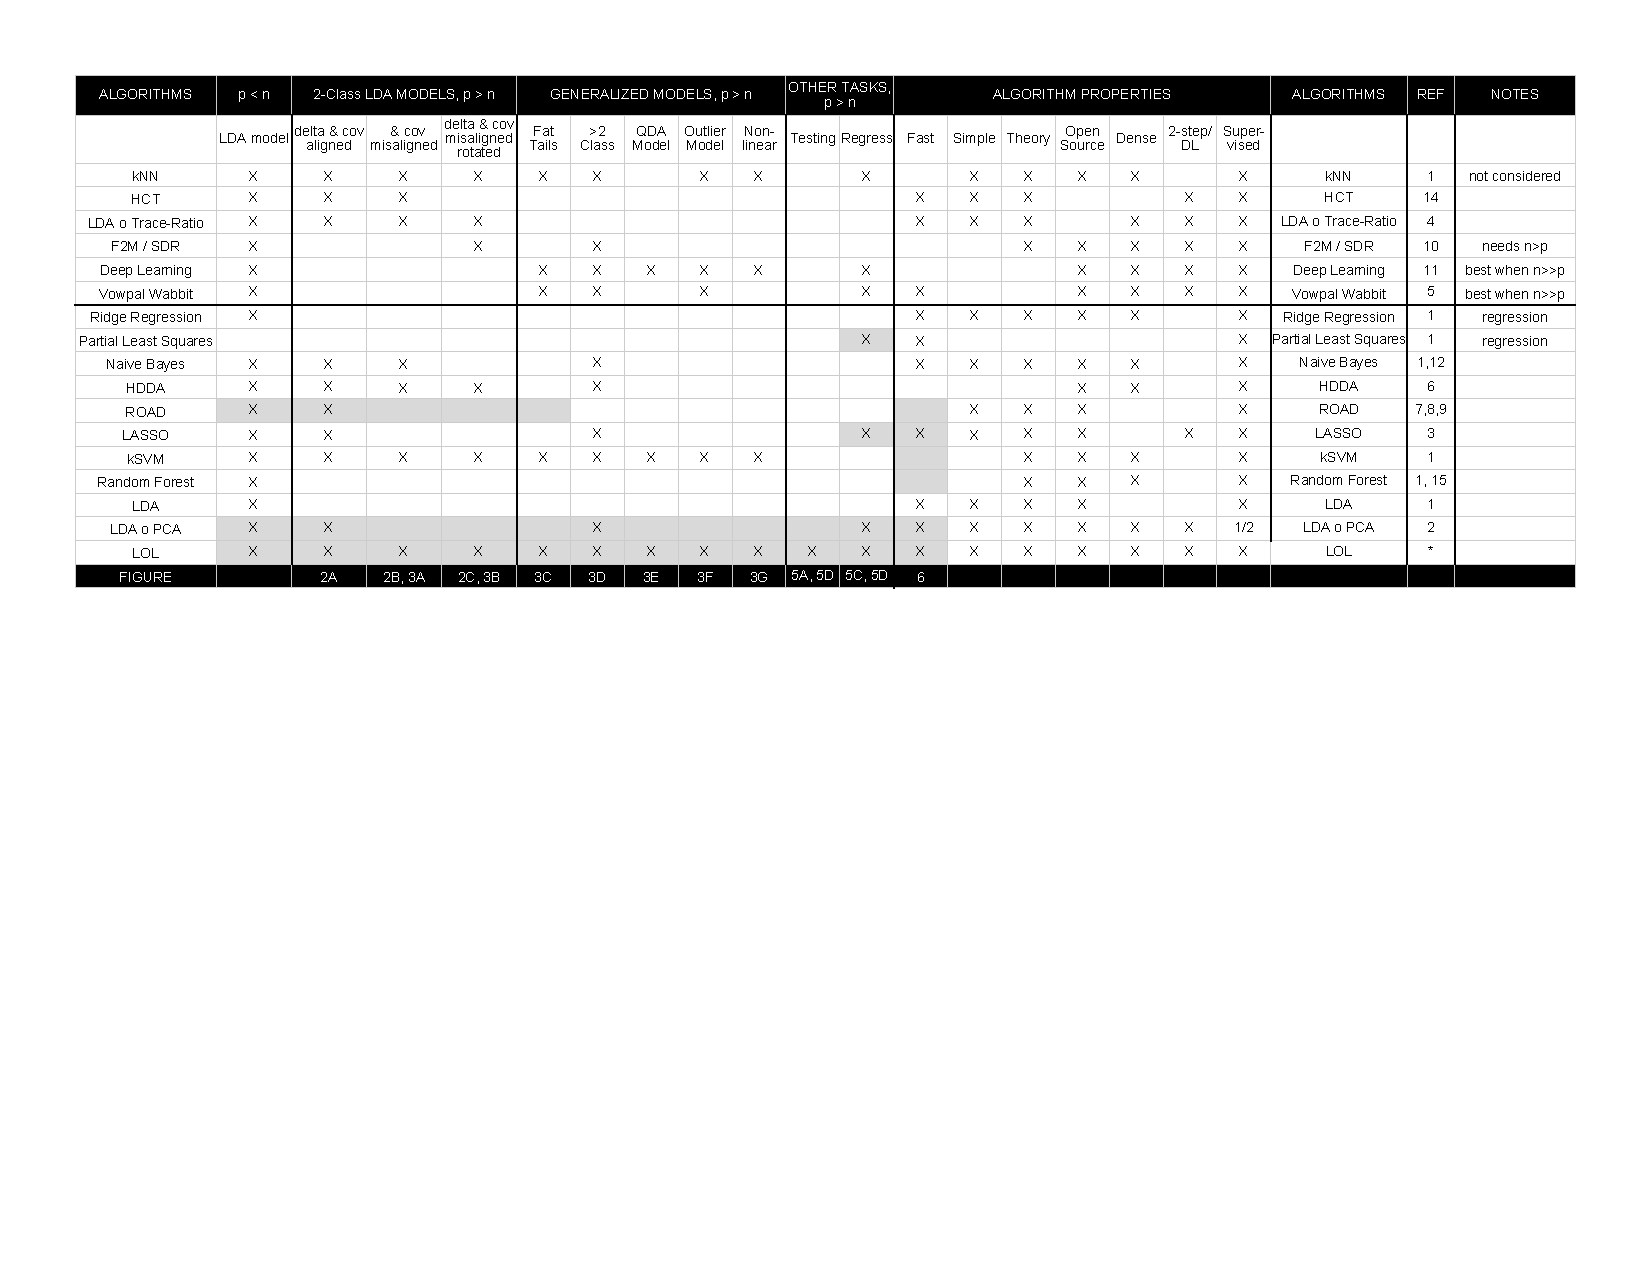
\includegraphics[width=1\linewidth,trim=0.5in 4.5in 0.5in 0.5in,clip=true]{../Figs/table} %l b r t
\caption{Table of algorithms and their properties for high-dimensional data. Gray elements indicate that results are demonstrated in the Figure labeled in the bottom row. 'X' denotes relatively good performance for a given setting, or has the particular property.
}
\label{f:table}
\end{figure}







\clearpage
\appendix
\section{Theoretical Background}


\subsection{The Classification Problem}

Let $(\bX,Y)$ be a pair of random variables, jointly sampled from $F :=F_{\bX,Y}=F_{\bX|Y}F_{Y}$.
Let $\bX$ be a multivariate vector-valued random variable, such that its realizations live in p dimensional Euclidean space, $\bx \in \Real^p$.  Let $Y$ be a categorical random variable, whose realizations are discrete,  $y \in \{0,1,\ldots C\}$.  The goal of a classification problem is to find a function $g(\bx)$ such that its output tends to be the true class label $y$:
\begin{align*} %\label{eq:bayes}
g^*(\bx) := \argmax_{g \in \mc{G}} \PP[g(\bx) = y].
\end{align*}
When the joint distribution of the data is known, then the Bayes optimal solution is:
\begin{align}  \label{eq:R}
g^*(\bx) := \argmax_y f_{y|\bx} = \argmax_y f_{\bx|y}f_y =\argmax_y \{\log f_{\bx|y} + \log f_y \}
\end{align}
Denote expected misclassification rate of classifier $g$ for a given joint distribution $F$,
\begin{align*}
L^F_g := \EE[g(\bx) \neq y] := \int \PP[g(\bx) \neq y] f_{\bx,y} d\bx dy,
\end{align*}
where $\EE$ is the expectation, which in this case, is with respect to $F_{XY}$.
For brevity, we often simply write $L_g$, and we define $L_* := L_{g^*}$.


\subsection{Linear Discriminant Analysis (\Lda)}

Linear Discriminant Analysis (\Lda) is an approach to classification that uses a linear function of the first two moments of the distribution of the data.  More specifically, let $\mu_j=\EE[F_{X|Y=j}]$ denote the class conditional mean, and let $\bSig=\EE[F_{X}^2]$ denote the joint covariance matrix, and $\pi_j=\PP[Y=j]$.   Using this notation, we can define the \Lda~classifier:
\begin{align*}
g_{\Lda}(\bx)&:=\argmin_y \frac{1}{2} (\bx-\bmu_0)\T \bSig^{-1}(\bx-\bmu_0) + \II\{Y=y\}  \log \pi_y,
\end{align*}
where $\II\{ \cdot\}$ is one when its argument is true, and zero otherwise.
Let $L_{\Lda}^F$ be the misclassification rate of the above classifier for distribution $F$.
%
Assuming equal class prior and centered means,  $\pi_0=\pi_1$ and $(\bmu_0+\bmu1)/2=\mb{0}$, re-arranging a bit, we obtain
\begin{align*}
g_{\Lda}(\bx) :=  \argmin_y \bx\T \bSig^{-1} \bmu_y.
\end{align*}
In words, the  \Lda~classifier chooses the class for whom the projection of an input vector $\bx$, onto $\bSig^{-1} \bmu_y$, is maximized.
%
When there are only two classes, this further simplies to
\begin{align*}
g_{2-\Lda}(\bx) :=  \II\{ \bx\T \bSig^{-1} \bdel > 0 \},
\end{align*}
where $\bdel=\bmu_0-\bmu_1$.   Note that the equal class prior and centered means assumptions merely changes the threshold constant from $0$ to something else.

\subsection{\Lda~Model}

A statistical model is  a family of distributions indexed by a parameter $\bth \in \bTh$, $\mc{F}_{\bth}=\{F_{\bth} : \bth \in \bTh \}$.
Consider the special case of the above where $F_{\bX|Y=y}$ is a multivariate Gaussian distribution,
$\mc{N}(\bmu_y,\bSig)$, where each class has its own mean, but all classes have the same covariance.
We refer to this model as the \Lda~model.
Let $\bth=(\bpi,\bmu,\bSig)$, and let $\bTh_{C-\Lda}=( \triangle_C, \Real^{p \times C},\Real_{\succ 0}^{p \times p})$, where $\bmu=(\bmu_1,\ldots, \bmu_C)$, $\triangle_C$ is the $C$ dimensional simplex, that is $\triangle_C = \{ \bx : x_i \geq 0 \forall i, \sum_i x_i = 1\}$, and $\Real_{\succ 0}^{p \times p}$ is the set of positive definite  $p \times p$ matrices. Denote
$\mc{F}_{\Lda}=\{F_{\bth} : \bth \in \bTh_{\Lda}\}$, dropping the superscript $C$ for brevity where appropriate.
The following lemma is well known:
\begin{lem}
$L_{\Lda}^F=L_*^F$ for any $F \in \mc{F}_{\Lda}$.
\end{lem}

\begin{proof}
Under the \Lda~model, the Bayes optimal classifier is available by plugging the explicit distributions into Eq.~\eqref{eq:R}.
\end{proof}




\section{Projection Based Classifiers}


Let $\bA \in \Real^{d \times p}$ be an orthonormal matrix, that is, a matrix that projects p dimensional data into a d dimensional subspace, where $\bA\bA\T$ is the $d \times d$ identity matrix, and $\bA\T \bA$ skis symmetric $p \times p$ matrix with rank d.   The question that motivated this work is: what is the best projection matrix that we can estimate, to use to ``pre-process'' the data prior to applying \Lda.
% \begin{lem}
% $g_{\Lda}^F(\bA \bx)= \II \{ (\bA \bx)\T \bSig^{-1}_A \bdel_A > 0\}$.
% \end{lem}
Projecting the data $\bx$ onto a low-dimensional subspace, and the classifying via \Lda~in that subspace is equivalent to redefining the parameters in the low-dimensional subspace,
$\bSig_A=\bA \bSig \bA\T \in \Real^{d \times d}$ and $\bdel_A = \bA \bdel \in \Real^d$, and then using $g_{\Lda}$.  When $C=2$, $\pi_0=\pi_1$, and $(\mu_0+\mu_1)/2=\mb{0}$, this amounts to:
\begin{align} \label{eq:g_A}
g^d_A(x) := \II \{ (\bA \bx)\T \bSig^{-1}_A \bdel_A > 0\}, \text{ where } \bA \in \Real^{d \times p}.
\end{align}
Let $L^d_A :=\int \PP[g_A(\bx)=y] f_{\bx,y} d\bx dy$.
Our goal therefore is to be able to choose $A$ for a given parameter setting $\bth=(\bpi, \bdel,\bSig)$, such that $L_A$ is as small as possible (note that $L_A$ will never be smaller than $L_*$).

Formally, we seek to solve the following optimization problem:
% \begin{align} \label{eq:A}
% \bA_* = \argmin_{\bA \in \Real^{p \times d}} L_A.
% \end{align}
\begin{equation} \label{eq:A}
\begin{aligned}
& \underset{\bA}{\text{minimize}}
& & \EE [ \II \{ \bx\T \bA\T \bSig^{-1}_A \bdel_A > 0\} \neq y] \\
& \text{subject to} & & \bA \in \Real^{p \times d}, \quad \bA \bA\T = \bI_{d \times d},
\end{aligned}
\end{equation}
where $\bI_{u \times v}$ is the $u \times v$ identity matrix identity, that is, $\bI(i,j)=1$ for all $i=j \leq \min(u,v)$, and zero otherwise.
Let $\mc{A}^d=\{\bA : \bA \in \Real^{d \times p}, \bA \bA\T = \bI_{d \times d}\}$, and let $\mc{A}_* \subset \mc{A}$ be the set of $\bA$  that minimize Eq.~\eqref{eq:A}, and let $\bA_* \in \mc{A}_*$ (where we dropped the superscript $d$ for brevity).   Let $L_{\bA}^*=L_{\bA_*}$ be the misclassification rate for any $\bA \in \mc{A}_*$, that is, $L_{\bA}^*$ is the Bayes optimal misclassification rate for the classifier that composes $\bA$ with \Lda.


In our opinion, Eq.~\eqref{eq:A} is the simplest supervised manifold learning problem there is: a two-class classification problem, where the data are multivariate Gaussians with shared covariances, the manifold is linear, and the classification is done via \Lda.
Nonetheless, solving Eq.~\eqref{eq:A} is difficult, because we do not know how to evaluate the integral analytically, and we do not know any algorithms that are guaranteed to find the global optimum in finite time.  This has led to previous work using a surrogate function \cite{not sure who}.
We proceed by studying a few natural choices for $\bA$.





\subsection{Bayes Optimal Projection}

% Let $\mb{\bA}\T=\bSig^{-1} \bdel$.
\begin{lem}
$\bdel\T  \bSig^{-1} \in \mc{A}_*$
\end{lem}

\begin{proof}
Let $\bB = (\bSig^{-1} \bdel)\T = \bdel\T (\bSig^{-1})\T = \bdel\T \bSig^{-1}$, so that $\bB\T = \bSig^{-1} \bdel$,
% = \bdel\T \bOm\T
and plugging this in to Eq.~\eqref{eq:g_A}, we obtain
\begin{align*}
g_{B}(x) &= \II \{ \bx \bB\T  \bSig^{-1}_{B} \bdel_{B} > 0\} &
\\&= \II \{ \bx\T \bSig^{-1} \bdel \times (\bSig^{-1}_{B} \bdel_{B}) > 0\} & \text{plugging in $\bB$}
\\&= \II \{ \bx\T \bSig^{-1} \bdel k > 0\} & \text{because $\bSig^{-1}_{B} \bdel_{B} > 0$}.
\end{align*}
In other words, letting $\bB$ be the Bayes optimal projection recovers the Bayes classifier, as it should.
Or, more formally, for any $F \in \mc{F}_{\Lda}$, $L_{\bdel\T \bSig^{-1}} = L_*$
\end{proof}

\subsection[PCA]{Principle Components Analysis (\Pca) Projection}

Principle Components Analysis (\Pca) finds the directions of maximal variance in a dataset.  \Pca~is closely related to eigendecompositions and singular value decompositions (\Svd).  In particular, the top principle component of a matrix $\bX \in \Real^{p \times n}$, whose columns are centered, is the eigenvector with the largest corresponding eigenvalue of the centered covariance matrix $\bX \bX\T$.  \Svd~enables one to estimate this eigenvector without ever forming the outer product matrix, because \Svd~factorizes a matrix $\bX$ into $\bU \bS \bV\T$, where  $\bU$ and $\bV$ are orthonormal  ${p \times n}$ matrices, and $\bS$ is a diagonal matrix, whose diagonal values are decreasing,  $s_1 \geq s_2 \geq \cdots > s_n$.  Defining $\bU =[\bu_1, \bu_2, \ldots, \bu_n]$, where each $\bu_i \in \Real^p$, then $\bu_i$ is the $i^{th}$ eigenvector, and $s_i$ is the square root of the $i^{th}$ eigenvalue of $\bX \bX\T$.  Let $\bA^{\Pca}_d =[\bu_1, \ldots , \bu_d]$ be the truncated \Pca~orthonormal matrix.

The \Pca~matrix is perhaps the most obvious choice of a orthonormal matrix for several reasons.  First, truncated \Pca~minimizes the squared error loss between the original data matrix and all possible rank d representations:
\begin{align*}
\argmin_{A \in \Real^{d \times p} : \bA \bA\T = \bI_{d \times d}} \norm{ \bX - \bA^T \bA }_F^2.
\end{align*}
Second, the ubiquity of \Pca~has led to a large number of highly optimized numerical libraries for computing \Pca~(for example, LAPACK \cite{Anderson1999a}).

Moreover, let $\bU_d=[\bu_1,\ldots,\bu_d] \in \Real^{p \times d}$, and note that $\bU_d\T \bU_d = \bI_{d \times p}$ and $\bU_d\T \bU_d  = \bI_{p \times d}$.  Similarly, let $\bU \bS \bU\T = \bSig$, and $\bU \bS^{-1} \bU\T = \bSig^{-1}$.  Let $\bS_d$ be the matrix whose diagonal entries are the eigenvalues, up to the $d^{th}$ one, that is $\bS_d(i,j)=s_i$ for $i=j \leq d$ and zero otherwise.  Similarly, $\bSig_d=\bU \bS_d \bU\T=\bU_d \bS_d \bU_d\T$.

Let $g_{\Pca}^d:=g_{A_{\Pca}^d}$, and let $L_{\Pca}^d:=L_{A_{\Pca}^d}$.
And let $g_{\Lda}^d := \II \{ x \bSig_d^{-1} \bdel > 0\}$ be the regularized \Lda~classifier, that is, the \Lda~classifier, but sets the bottom $p-d$ eigenvalues to zero.

\begin{lem}
$L_{\Pca}^d = L_{\Lda}^d$.
\end{lem}

\begin{proof}
Plugging $\bU_d$ into Eq.~\eqref{eq:g_A} for $\bA$, and considering only the left side of the operand, we have
\begin{align*}
(\bA \bx)\T \bSig^{-1}_A \bdel_A &= \bx\T \bA\T \bA \bSig^{-1} \bA\T \bA \bdel,
\\&= \bx\T  \bU_d\bU_d\T \bSig^{-1} \bU_d\bU_d\T \bdel,
\\&= \bx\T  \bU_d \bU_d\T \bU \bS^{-1} \bU \bU_d\bU_d\T \bdel,
\\&= \bx\T  \bU_d \bI_{d \times p} \bS^{-1} \bI_{p \times d} \bU_d\T \bdel,
\\&= \bx\T  \bU_d \bS^{-1}_d  \bU_d\T \bdel ,
\\&= \bx\T  \bSig^{-1}_d  \bdel.
\end{align*}
\end{proof}

The implication of this lemma is that if one desires to implement Fisherfaces, rather than first learning the eigenvectors and then learning \Lda, one can instead directly implement regularized \Lda~by setting the bottom $p-d$ eigenvalues to zero.




\subsection[LOL]{Linear Optimal Low-Rank (\Lol) Projection}


The basic idea of \Lol~is to use both $\bdel$ and the top $d$ eigenvectors.  Most na\"ively, we could simply concatenate the two, $\bA_{\Lol}^d=[\bdel,\bA_{\Pca}^{d-1}]$.
Recall that eigenvectors are orthonormal.  To maintain orthonormality, we could easily apply Gram-Schmidt,  $\bA_{\Lol}^d=$ \sct{Orth}$([\bdel, \bA_{\Pca}^{d-1}])$.
Both in practice and in theory (as will be shown below), this orthogonalization step does not matter much.

to ensure that they are balanced appropriately, we normalize $\bdel$

each vector in $\bdel$ to have norm unity.  Formally, let $\mt{\bdel}_j = \bdel_j / \norm{\bdel_j}$, where $\bdel_j$ is the $j^{th}$ difference of the mean vector (remember, the number of vectors is equal to $C-1$, where $C$ is the total number of classes), and let  $\bA_{\Lol}^d=[\mt{\bdel}, \bA_{\Pca}^{d-(C-1)}]$.
The eigenvectors are all normalized and orthogonal to one another; to impose orthogonality between $\mt{\bdel}$ and the eigenvectors, we could use any number of numerically optimized algorithms.  However, in practice, orthogonalizing does not matter very much, so we do not bother. We formally demonstrate this below.




\section{Theoretical Properties of LDA based Classifiers}


\subsection{\Lda~is rotationally invariant}

For certain classification tasks, the ambient coordinates have intrinsic value, for example, when simple interpretability is desired.  However, in many other contexts, interpretability is less important \cite{Breiman2001b}.  When the exploitation task at hand is invariant to rotations, then we have no reason to restrict our search space to be sparse in the ambient coordinates, rather, for example, we can consider sparsity in the eigenvector basis.  Fisherfaces is one example of a rotationally invariant classifier, under certain model assumptions.
Let  $\bW$ be a rotation matrix, that is $\bW \in \mc{W}=\{\bW : \bW\T = \bW^{-1}$ and det$(\bW)=1\}$.
Moreover, let $\bW \circ F$ denote the distribution $F$ after transformation by an operator $\bW$.  For example, if $F=\mc{N}(\bmu,\bSig)$ then $\bW \circ F=\mc{N}(\bW  \bmu, \bW \bSig \bW\T)$.

\begin{defi}
A rotationally invariant classifier has the following property:
$$L_g^F = L_g^{W \circ F}, \qquad F \in \mc{F}.$$
In words, the Bayes risk of using classifier $g$ on distribution $F$ is unchanged if $F$ is first rotated, for any $F \in \mc{F}$.
\end{defi}


Now, we can state the main lemma of this subsection:  \Lda~is rotationally invariant.
\begin{lem} \label{l:rot}
$L_{\Lda}^F = L_{\Lda}^{W \circ F}$, for any $F \in \mc{F}$.
\end{lem}

\begin{proof}
\Lda~simply becomes thresholding $\bx\T \bSig^{-1} \bdel$.  Thus, we can demonstrate rotational invariance by demonstrating that $\bx\T \bSig^{-1} \bdel$ is rotationally invariant.

% First, note that for any distribution $F \in \mc{F}_{\Lda}$, we can reparameterize it such that $\bSig$ is diagonal.  This follows because for any $\bSig$, we can represent it as $\bSig=\bU \bS \bU$, and there exists a $\bW$ such that
% from the following:
% \begin{align}
% \bSig = \bU \bS \bU =
% \end{align}

\begin{align*}
% \bx\T \bSig^{-1} \bdel &=
(\bW \bx) \T  (\bW \bSig \bW\T )^{-1} \bW \bdel  %& \text{from Lemma \ref{l:rot}}\\
&= \bx\T \bW\T  (\bW \bU \bS \bU\T \bW\T)^{-1} \bW \bdel & \text{by substituting $\bU \bS \bU\T$ for $\bSig$} \\
&= \bx\T \bW\T  (\mt{\bU} \bS \mt{\bU}\T)^{-1} \bW \bdel & \text{by letting $\mt{\bU}=\bW \bU$} \\
&= \bx\T \bW\T  (\mt{\bU} \bS^{-1} \mt{\bU}\T) \bW \bdel & \text{by the laws of matrix inverse} \\
&= \bx\T \bW\T  \bW \bU \bS^{-1}  \bU\T \bW\T \bW \bdel & \text{by un-substituting $\bW \bU=\mt{\bU}$} \\
&= \bx\T  \bU \bS^{-1}  \bU\T  \bdel  & \text{because $\bW\T \bW = \bI$} \\
&= \bx\T   \bSig^{-1} \bdel & \text{by un-substituting $\bU \bS^{-1} \bU\T = \bSig$}
\end{align*}
\end{proof}

One implication of this lemma is that we can reparameterize without loss of generality.  Specifically, defining $\bW := \bU\T$ yields a change of variables: $\bSig \mapsto \bS$ and $\bdel \mapsto \bU\T \bdel := \bdel''$, where $\bS$ is a diagonal covariance matrix.  Moreover, let $\bd=(\sigma_1,\ldots, \sigma_D)\T$ be the vector of eignevalues, then $\bS^{-1} {\bdel'}=\bd^{-1} \odot \mt{\bdel}$, where $\odot$ is the Hadamard (entrywise) product.  The \Lda~classifier may therefore be encoded by a unit vector, $\mt{\bd}:= \frac{1}{m} \bd^{-1} \odot \mt{\bdel'}$, and its magnitude, $m:=\norm{\bd^{-1} \odot \mt{\bdel}}$.
This will be useful later.




\subsection[]{Rotation of Projection Based Linear Classifiers $g_A$}

By a similar arguement as above, one can easily show that:

\begin{align*}
(\bA  \bW \bx) \T  (\bA \bW  \bSig  \bW\T \bA\T)^{-1} \bA \bW \bdel
&= \bx\T (\bW\T \bA\T) (\bA \bW) \bSig^{-1} (\bW\T \bA\T) (\bA \bW) \bdel \\
&= \bx\T \bY\T \bY \bSig^{-1} \bY\T \bY \bdel \\
&= \bx\T \bZ \bSig^{-1} \bZ\T \bdel \\
&= \bx\T (\bZ \bSig \bZ\T)^{-1} \bdel = \bx\T \mt{\bSig}_d^{-1} \bdel,
% (\bA\T \bA \bx) \T  \bSig^{-1} \bA\T \bA \bdel = (\bA \bx)\T \bSig^{-1}_A \bdel_A.
\end{align*}
% \end{proof}
where $\bY = \bA \bW \in \Real^{d \times p}$ so that $\bZ=\bY\T \bY$ is a symmetric ${p \times p}$ matrix of rank $d$.  In other words, rotating and then projecting is equivalent to a change of basis.
The implications of the above is:
\begin{lem}
$g_A$ is rotationally invariant if and only if span($\bA$)=span($\bSig_d$).
In other words, \Pca~is the only rotationally invariant projection.
\end{lem}





\subsection{Simplifying the Objective Function}

Recalling Eq.~\eqref{eq:g_A}, a projection based classifier is effectively thresholding the dot product of $\bx$ with the linear projection operator $\bP_A :=\bA\T \bSig_A^{-1} \bdel_A \in \Real^p$, and let $\bP_*:=\bP_{\bA_*}$.  Unfortunately, the nonlinearity in in Eq.~\eqref{eq:A} makes analysis difficult.
However, because of the linear nature of the classifier and projection matrix operator, an objective function that is simpler to evaluate is available.
Define
$\angle(\bP,\bP') = \frac{ \bP\T \bP'}{||\bP||_2 ||\bP'||_2} \in (0,1)$, and consider

\begin{equation} \label{eq:angle}
\begin{aligned}
& \underset{\bA}{\text{minimize}}
& & -\angle(\bP_A,\bP_*),
\\ & \text{subject to} & & \bA \in \Real^{p \times d}, \quad \bA \bA\T = \bI_{d \times d}.
\end{aligned}
\end{equation}

\begin{lem} \label{l:angle}
The solution to Eq.~\eqref{eq:angle} is also the solution to Eq.~\eqref{eq:A} for any given $d$.
\end{lem}

\begin{proof}
The minimum of Eq.~\eqref{eq:angle} is clearly $\bA=\bSig^{-1} \bdel$, which is also the minimum of Eq.~\eqref{eq:A}.
\end{proof}


\begin{remark}
$\angle$ is merely the angle between two vectors, and is therefore scale invariant.  In other words, $\angle(\bP_A,\bP)=\angle(\bP_{c A},\bP)$, for any $c > 0$.
\end{remark}

Given the above, we can evaluate various choices of $\bA$ in terms of their induced projection operator $\bP_A$ and the angle between said projection operators and the Bayes optimal projection operator.
% Let $\bP_*=\bP_{A_*}=\bSig^{-1} \bdel$,
% and $\alpha^*_A=\angle(\bP_*,\bP_A)$.


\begin{lem}
$\angle(\bP_A, \bP_*) <1  \implies L_A > L_*$
\end{lem}


\begin{proof}
If $\angle(\bP_A, \bP_*) <1$, then there exists an $\bx$ such that $\II\{ \bx\T \bP_A >0 \} \neq \II\{ \bx\T \bP_* >0 \}$, and therefore, $L_A > L_*$.
\end{proof}



\begin{conj}
% \begin{lem}
\label{q:a2}
$$\angle(\bP_A,\bP_*) \leq \angle(\bP_B,\bP_*) \implies L_A \leq L_B.$$
% \end{lem}
\end{conj}



% Note that Conjecture \ref{q:a2} is a stronger statement than Conjecture \ref{q:a1}, and in particular, if Conjecture \ref{q:a2} is true, then so is Conjecture \ref{q:a1}.




\subsubsection{When $d=1$}

\begin{remark}
If $\bA \in \mc{A}_*$ and $\bB \notin \mc{A}_*$, then $\angle(\bA\T,\bA_*\T)=1$ and $\angle(\bB\T,\bP_*\T)<1$, and therefore $\angle(\bA\T,\bA_*\T) > \angle(\bB\T,\bA_*\T)$.
\end{remark}



\begin{conj} \label{q:angle}
When $d=1$:
% \begin{lem}
\label{q:a1}
$$\angle(\bA\T,\bA_*\T) \leq \angle(\bB\T,\bA_*\T) \implies \angle(\bP_A,\bP_*) \leq \angle(\bP_B,\bP_*).$$
% \end{lem}
\end{conj}

\begin{proof}
I believe so, but i don't see how to prove it. A little arithmetic shows that the left hand side means that:
$$\bA \bSig^{-1} \bdel > \bB \bSig^{-1} \bdel.$$

Similarly, the right hand side means that:
$$\bdel \bA\T \bA \bSig^{-1} \bA\T a > \bdel \bB\T \bB \bSig^{-1} \bB\T b,$$
where we substituted $a:=\bA\bSig^{-1} \bdel$ and $b:=\bB \bSig^{-1} \bdel$.

But I do not see how to go any further.
\end{proof}



\newpage
\subsection{\Pca~versus \Lol} \label{sec:pvl}


We would like to prove that \Lol~is always better than \Pca, when using one or the other to project the data onto a low dimensional space, followed by classifying with \Lda, under a wide variety of of settings.  Formally, we would like to prove $\PP[L_{\Lol}^d \leq L_{\Pca}^d]$ is big.  To do so, we ask a sequence of increasingly sophisticated questions that have the following form:
\begin{compactenum}
\item Under which parameter settings is \Lol~better than \Pca?
\item How often do those parameter settings arise, under various statistical models of the parameters?
\end{compactenum}


Recall that for the $C$-class classification problem, the parameter from which we sample the data is $\bth_c=(\pi_c,\bmu_c,\bSig_c)$, where

\begin{compactitem}
\item the class probabilities are non-negative and sum to unity: $\bpi=(\pi_1,\ldots,\pi_C) \in \triangle_C := \sum_{c \in \mc{C}} \pi_c = 1$ and $\pi_c \geq 0 \forall c \in \mc{C}$,
\item the class means are $p$-dimensional vectors: $\bmu_c \in \Real^{p}$ is the class $c$ mean vector, and
\item the class covariances are positive definite $p \times p$ real matrices: $\bSig_c  \in \Real^{p \times p}_+$ is the class conditional covariance matrix (and $\Real^{p \times p}_+$ is the set of positive definite real $p\times p$ matrices).
\end{compactitem}

The fully unconstrained parameter space is therefore $\bTh=\{ \triangle_C \times (\Real^p, \Real^{p \times p}_+)^C \}$.

When using a projection based classifier, we also have the hyperparameter $d$ which specifies the the dimensionality of the low-dimensional projection.

We thus try to answer the above two questions for increasingly relaxed constraints on the parameter space and $d$. To start, we assume that:
\begin{compactenum}
\item we have only two classes, $C=2$;
\item each class has the same covariance matrix, $\bSig_0=\bSig_1$.
\end{compactenum}

For simplicity (but without loss of generality), we will also assume that the two classes have centered means and equal priors, that is, $(\bmu_0+\bmu_1)/2=0$ and $\pi_0=\pi_1=1/2$ (relaxing this assumption merely changes the threshold of the classifier).  Let the parameter space defined by these constraints be denoted $\bTh' = \{\Real^{2p}, \Real_+^{p \times p} \}$. In Section \ref{sec:pvl}, we will always assume $\bth \in \bTh'$, unless otherwise specified.

Given the above, we consider the following sequence of relaxations, first when $d=1$, and then when $d < p$:
\begin{compactenum}
\item the covariance is a scaled identity matrix, that is, $\bSig=k \mb{I}$;
\item the covariance is a diagonal matrix, that is, $\bSig=\bS$, where $\bS_{ij}=\sigma_i$ when $i=j$ and is zero otherwise;
\item the covariance is an arbitrary positive definite matrix, that is  $\bSig \in \Real^{p \times p}_\succ$.
\end{compactenum}

After those, extensions to the multiclass and/or different covariance matrix setting might then also be explored.








\subsubsection{$d=1$}

In this section, we will only consider $d=1$, meaning that
\begin{compactitem}
\item \Lol~is simply $\bdel$,
\item \Pca~is simply $\bu_1$, the eigenvector corresponding to the largest eigenvalue of $\bSig$.
\end{compactitem}



\paragraph{Scaled Identity Covariance Matrix}


\begin{lem}
\Lol~better than \Pca~almost always when $\bSig=k \mb{I}$.
\end{lem}

\begin{proof}
To prove this statement, we first show how to define $\bA_{\Lol}^1$ and $\bA_{\Pca}^1$ is this setting.

\begin{compactitem}
\item $\bA_{\Lol}^1$ is simply $\bdel$, regardless of the covariance matrices and priors.
\item When $\bSig=k \bI$, $\bA_{\Pca}^1$ is a random vector, because the first principal component of a scaled identity matrix can equally be defined as any basis vector.
\end{compactitem}

Thus, only when the first eigenvector of the covariance matrix is randomly assigned to $\bdel$ will \Pca~work as well as \Lol.
\end{proof}


Given the conditions under which \Lol~is better than \Pca, we next ask how often that happens, under a reasonable model assumption.

\begin{lem}
$\PP[L_{\Lol}^1 \leq L_{\Pca}^1]=1$ when $\bSig=k \bI$ and $\bdel \sim \mc{N}(\bmu_{\delta},\bSig_{\delta})$.
\end{lem}

\begin{proof}
When $\bdel \sim \mc{N}(\bmu_\delta,\bSig_\delta)$, the probability that it exactly equals any vector $\bx \in \Real^d$ is real, this includes, of course,  $\bu_1$, the first eigenvector of $k \mb{I}$.  Thus, $\PP[\bdel \propto \bu_1]=0$, no matter how $\bu_1$ is chosen (as long as it is not chosen using the knowledge of the value of $\bdel$).
This implies that $\PP[\angle(\bu_1\T,\bA_*\T) =1 ] = 0$, and therefore, $\PP[L_{\bu_1} \geq L_*] =1$.
\end{proof}


% \newpage
\paragraph{Diagonal covariance matrix}



Now consider a simple generalization of the above scenario, namely, $\bSig=\bS$ is diagonal.
We want to know under what conditions is \Lol~better than \Pca, and how often that happens under a reasonable model.


Let $\bs$ be the singular values of $\bSig$.  When $\bSig$ is diagonal, its diagonal elements are $s_1,\ldots,s_p$, and we call that matrix $\bS$.
Recalling that $s_i=\lambda_i^2$, where $\lambda_i$'s are eigenvalues, and when a matrix is diagonal, $s_i=\lambda_i^2$, we have  $\bA_*=\bS^{-1} \bdel=\bs^{-1} \odot \bdel := \mt{\bdel} =(\del_1/\lambda_1^2,\ldots,\del_p/\lambda_p^2)$.



\begin{lem}
\Lol~is better than \Pca~whenever $1-\delta_1 < {s_1}/{\delta_1} \sum_{i=2}^p {\delta_i^2}/{s_i}$.
A consequence of this is that \Lol~is always better than \Pca~whenever $\delta_1>1$.
This means that when the variables are independent
\end{lem}

% \begin{question}
% When is $\angle(\bdel,\mt{\bdel}) > \angle(\bu_1, \mt{\bdel})$?
% \end{question}


\begin{proof}
Recalling that $\bu_i=\be_i$, where $\be_i$ is a vector of all zeros except a one in the $i^{th}$ element, and let $\bu^i=\bu_i$ for simplicity here, we can show that:
$$
\angle(\bdel,\mt{\bdel}) =
\sum_i \delta_i \mt{\delta}_i =
\sum_i \delta_i s^{-1}_i \delta_i =
\sum_i \delta_i^2 / s_i
$$
and
$$
\angle(\bu^1, \mt{\bdel})  = \sum_i u^1_i \mt{\delta_i} =  \sum_i u^1_i s^{-1}_i {\delta_i}= \sum_i u^1_i {\delta_i} /s_i =  u^1_1 {\delta_1} /s_1=  {\delta_1} /s_1.
$$

Thus, $\angle(\bdel,\mt{\bdel}) > \angle(\bu_1, \mt{\bdel})$ any time that
$\sum_i \delta_i^2 / s_i > \delta_1 / s_1$.
Note that at a minimum, it must be that $\delta_1 < 1$.

Conjectures 1 and 2 demonstrate that if the angle is better, than Bayes error is also better, and this completes the proof.
\end{proof}

% By definition, $\bA_{\Lol}^1=\bdel$, and $\bA_{\Pca}^1=\bu_1$, where $\bu_1$ is the eigenvector associated with the largest eigenvalue of $\bS$.

% We consider a simple version of our question: how often is the angle between $\bA_{\Lol}^1$ and $\bA_*$ bigger than the angle between $\bA_{\Pca}^1$ and $\bA_*$.  Formally, we would like to prove:



If Conjecture 1 and 2 are true, then the above also implies that \Lol's Bayes error is also better than \Pca's, in this setting.
Numerical experiments suggest this is true, and moreover, that when randomly sampling $\bdel$ and $\bS$, \Lol~always does better than \Pca.

% It would be nice to be able to show, immediately, that because $\bdel$ is closer to $\mt{\delta}$ than $\bu_1$ is, that their corresponding $\bP$ matrices and classification performance are also closer to the Bayes optimal.  Numerical results suggest this is true, but I do not know how to prove it yet.

% \begin{conj}
% $\PP[ \angle(A_{\Lol}^1,\bA_*)  \geq  \angle(\bA_{\Pca}^1,\bA_*)]=1$ for any $\bth \in \bTh_{2-\Lda}$.
% \end{conj}

% \begin{proof}
% coming soon.  numerical experiments are convincing.
% \end{proof}


\begin{conj}
\Lol~is almost always better than \Pca~whenever $s_i \iid \mc{U}(0,1)$ and $\delta_i \iid \mc{N}(0,1)$ for all $i \in [p]$.
% When $\bdel \sim \mc{N}(\bmu_\delta, \bSig_\delta)$ and $\bs \sim \log \mc{N}(\bmu_s,\bSig_s)$, $\PP[\sum_i \delta_i^2 / s_i > \delta_1 / s_1]=1$.
\end{conj}
\begin{proof}
We start with the very simple scenario of $p=1$ and condition on $s$ to build intuition.
In this setting we have:
\begin{align}
\PP[ \delta^2 / s > \delta/s ] = \PP[ \delta^2 / s - \delta/s  > 0].
\end{align}
Let $z= x+y$, where $x= \frac{\delta^2}{s}$  and $y=\frac{\delta}{-s}$.
So, $x$ has a generalized chi-squared distribution and $y$ has a normal distribution.
A bit of algebra reveals the explicit form of this distribution, however, it includes an integral that we do not know how to evaluate.  Thus, instead of solving exactly for the above, we provide a bound.

Bennett's inequality states given $X_1,\ldots, X_n$, assume:
\begin{compactitem}
\item each $X_i$ is independent of all others
\item (without loss of generality) $\EE[X_i]=0 \forall i$
\item $|X_i|<a$ almost surely for all $i$
\item $\sigma^2 = \frac{1}{n} \sum_i \VV(X_i)$.
\end{compactitem}
Then, for any $t \geq 0$

% $$ \PP[ \sum_i X_i > t] \leq \exp \left{ -\frac{n\sigma^2}{a^2} h \left( \frac{at}{n\sigma^2}\right) \right}, $$
where $h(u)=(1+u) \log (1+u) - u$.

Recalling that $\VV(\sum_i X_i) = \sum_i \VV(X_i)$ for independent random variables, and that
\begin{compactenum}
\item  $\VV(\delta/s) = s^{-2}$
\item $\VV(\delta^2/s) = h(s)$
\end{compactenum}





where $\Phi$ is the cumulative distribution function for a standard normal random variable.

Note that re-introducing randomness into $s$


Coming soon.  ``almost always'' and ``better'' mean with probability 1 and better in the sense of the angle between $\bA_{\Lol}^1$ and the Bayes vector is larger than that of $\bA_{\Pca}^1$ and the Bayes vector.
I believe this also implies Bayes error is better, but we have not yet shown that.
\end{proof}




\paragraph{Arbitrary Covariance Matrix}


\subsubsection{$d \geq 1$}
\subsubsection{Scaled Identity Covariance Matrix}
\subsubsection{Diagonal Covariance Matrix}
\subsubsection{Arbitrary Covariance Matrix}




\newpage
\section{Asymptotic Theory}

In real data problems,  the true joint distribution is unknown. Instead, what is provided is a set of training data.  We therefore assume the existence of $n$ training samples, each of which has been sampled identically and independently from the same distribution, $(\bX_i,Y_i) \iid F_{\bX,Y}$, for $i =1,2,\ldots, n$.  We can use these training samples to then estimate $f_{x|y}$ and $f_y$.  Plugging these estimates in to Eq.~\eqref{eq:bayes}, we obtain the Bayes plugin classifier:
\begin{align} \label{eq:plugin}
\mh{g}^*_n(\bx) := \argmax_y \mh{f}_{\bx|y}\mh{f}_y.
\end{align}
Under suitable conditions, it is easy to show that this Bayes plugin classifiers performance is asymptotically optimal.
Formally, we know that:
% \begin{align} \label{eq:pc}
$L_{\mh{g}^*_n} \conv L_{g^*}$.
% \end{align}


When the parameters, and we want to use a linear approach, we can implement a Bayes plug-in \Lda, which we call Fisher's Discriminant Analysis (\Fld) \cite{Fisher1925a}.  Under the two-class, equal prior, and centered means assumption, we have
% $\bSig$ and $\bdel$ are unknown, as in real data scenarios, we can use the training samples to estimate them, and plug them in, as in Eq.~\eqref{eq:plugin}:
\begin{align}
\mh{g}^*_n(\bx) := \II\{ \bx\T \mh{\bSig}^{-1} \mh{\bdel} > 0 \},
\end{align}
and $L_{\mh{g}_n}$ is the misclassification rate for an estimated classifier, $\mh{g}_n$.
% This Bayes plugin classifier is called Fisher's Linear Discriminant (FLD; in contrast to \Lda, which uses the true---not estimated---parameters).
Unfortunately, when $p \gg n$, the estimate of the covariance matrix $\bSig$ will be low-rank, and therefore, not invertible (because an infinite number of solutions all fit equally well).  In such scenarios, we seek alternative methods, even in the \Lda~model.

We would like to prove:
\begin{lem}
$L_{\mh{\Lol}}^d \conv L_*$ for any $\bth \in \bTh'$.
\end{lem}


\begin{lem}
$\PP[L_{\mh{\Pca}}^d \conv L_*]>0$ for any $\bth \in \bTh'$
\end{lem}

\newpage
\section{Finite Sample Theory}

It would be awesome to prove something like:
\begin{thm}
\begin{align*}
\PP[ \mh{L}_{\Lol}^d - \mh{L}_{\Pca}^2  > 0  ] < f(\bth,d,n),
\end{align*}
\end{thm}
which would state that \Lol~is better than \Pca, again, under suitable assumptions.


\begin{thm}
\begin{align*}
\PP[ \bP_{\Pca} \T \bP_*  - \bP_{\Lol} \T \bP_*  > t \norm{\bP_A} \norm{\bP_*} ] < f(t,p,d),
\end{align*}
\end{thm}
which would state that \Lol~is better than \Pca, again, under suitable assumptions.

In terms of distributiosn of the above, it seems that perhaps we could start simple.
Assume for the moment that $\bdel,\bu_1,\ldots,\bu_p \iid \mc{N}(\bmu_p, \bSig_p)$, and let $\bLam=(\bu_1,\ldots,\bu_p)\T$, and $\bSig = \bLam\T \bLam$.

The reason the above is probabilistic is because it is under certain assumptiosn on the \emph{distributions} of $bdel$, $\bSig$, and $\bA$.


Perhaps even simpler is to start with specific assumptions about $\bdel$, $\bSig$, and $\bA$. Because \Lda~is rotationally invariant, I believe that we can assert, without loss of generality, that $\bSig=\bS$, where $\bS$ is a diagonal matrix with diagonal entries $\sigma_1,\ldots, \sigma_p$, where all $\sigma_j > 0$.
Now, the optimal projection $\bSig^{-1} \bdel$ is just a simple dot product,  $\bd\T \bdel$, where $\bd=$diag($\bS$)$\in \Real^p$.


For example, letting $\bA=\bU_d$, and letting $\bU_i=e_i$ be the unit vector, with zeros everywhere except a one in the $i^{th}$ position,  we have
\begin{align*}
\bP_A\T \bP_* %&
= \bdel\T \bU_d\T \bU_d \bSig^{-1} \bU_d\T \bU_d \bSig^{-1} \bdel %\\ =
\bdel\T \bSig_d \bSig^{-1} \bSig_d \bSig^{-1} \bdel %\\&
= \bdel\T \bSig^{-2} \bdel.
\end{align*}


% Consider $\bP_*:=\bP_{\bA_*}$ and $\bP_{\Pca_d} := \bP_{A^{\Pca}_d}$.
% Now, consider $\alpha_{\Pca} := \angle (\bP_*, \bP_{\Pca_d})$.
% We would like to understand scenarios for which $\angle^*_{\Pca_d}$ is small, and when it is big.




% Note that this angle is a random variable, as it is a function of the sampled data $(\bX_i,Y_i) \iid P$.
So, we want to understand the probability that $\alpha_{\Pca}$ is small under different parameter settings, $\bth \in \bTh$.

% First note that

% \begin{lem}
% $\bP_A = \bP_{WA}$, when $\bW \T \bW = \bI$.
% \end{lem}


% \begin{proof}
% blah
% \end{proof}

\clearpage
% \bibliography{biblol}
\bibliography{../../../../Other/latex/library.bib}
\bibliographystyle{IEEEtran}


\end{document}
